\section*{Appendix}
\addcontentsline{toc}{section}{Appendix}

\subsection*{Appendix 1, Results (2.3.1) Scenarios: Sumo visuals}
\addcontentsline{toc}{subsection}{Appendix 1, Results (2.3.1) Scenarios: Sumo visuals}

This appendix contains the Sumo visuals for the traffic scenarios presented in part 2.3.1. \\

\begin{figure}[h]
\subsubsection*{(a): 1 traffic light, 2 phases, 2x2 incoming lanes.}
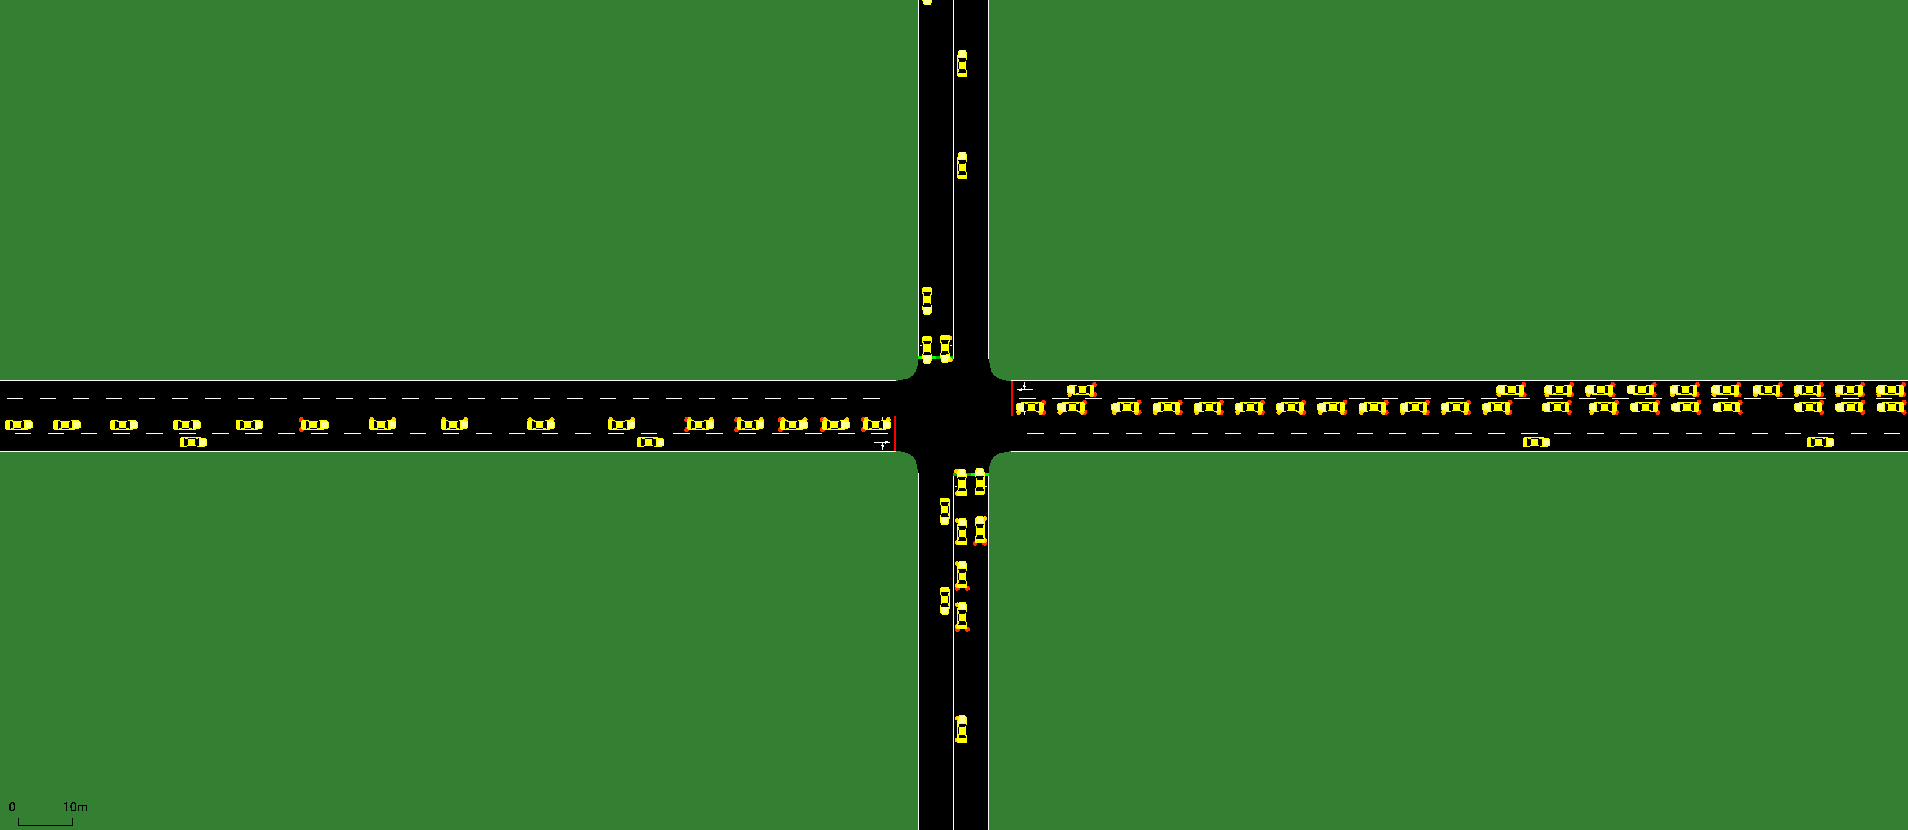
\includegraphics[width=\textwidth]{img/Appendix/scenario_a.png}
\centering
\end{figure}

\begin{figure}[h]
\subsubsection*{(b): 1 traffic light, 4 phases, 3x3 incoming lanes.}
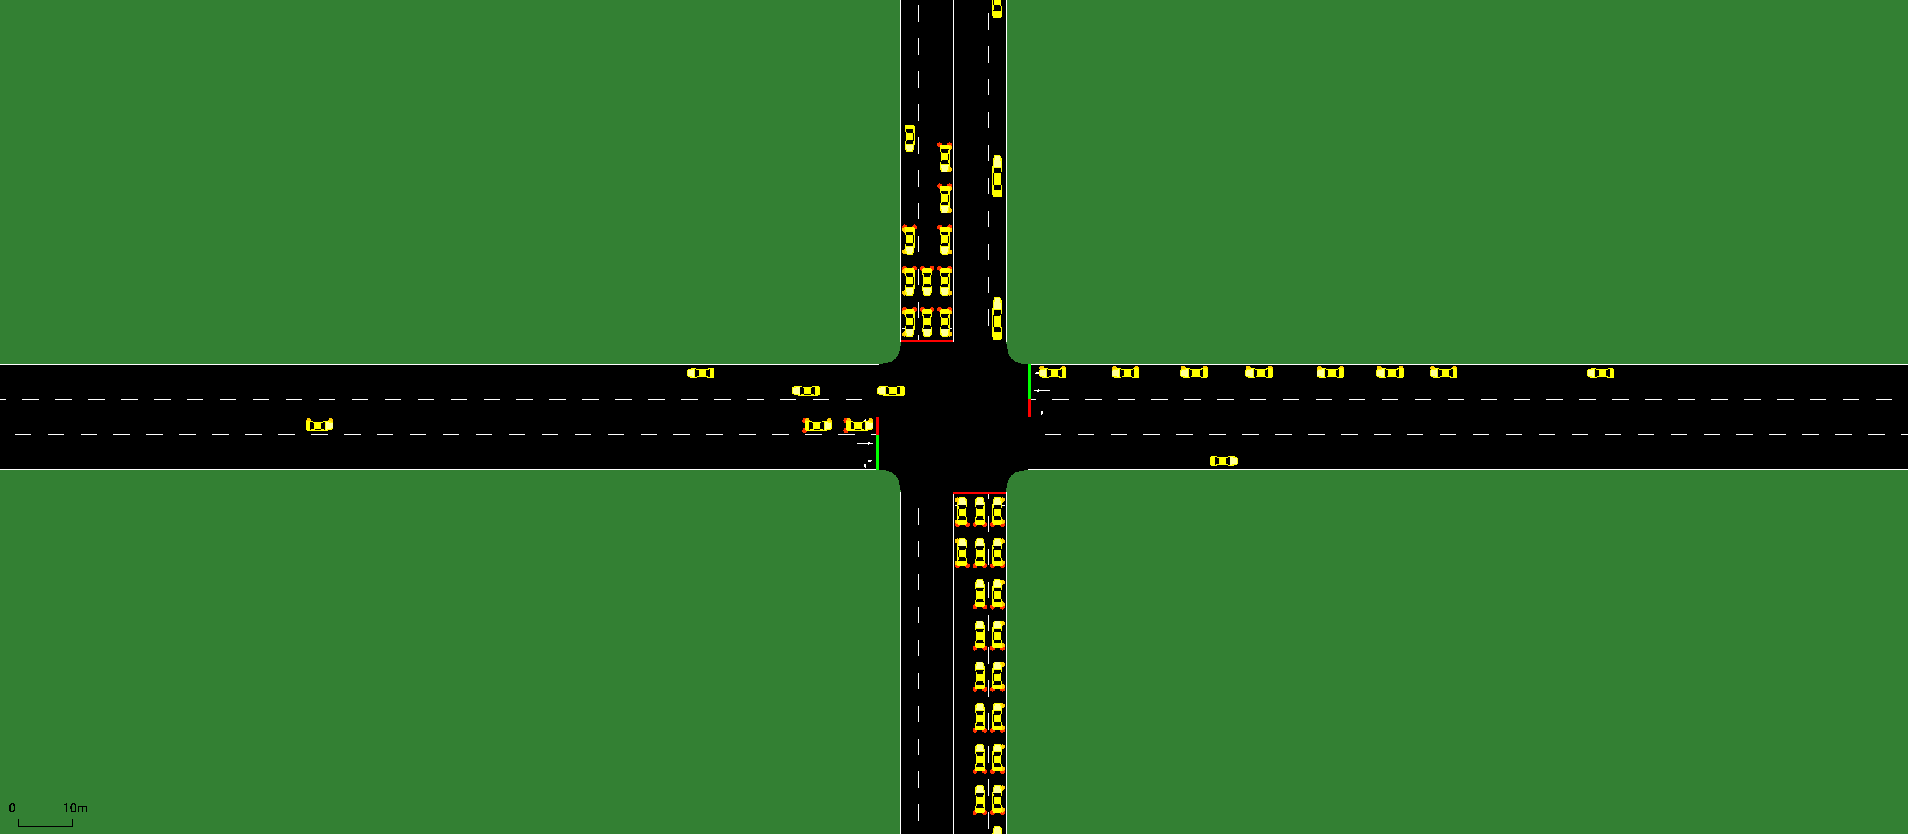
\includegraphics[width=\textwidth]{img/Appendix/scenario_b.png}
\centering
\end{figure}

\pagebreak

\newgeometry{left= 3cm, right= 2cm, bottom= 0cm, top= 2.6cm}

\begin{figure}[h]
\subsubsection*{(c): 1 traffic light, 4 phases, 4x4 incoming lanes.}
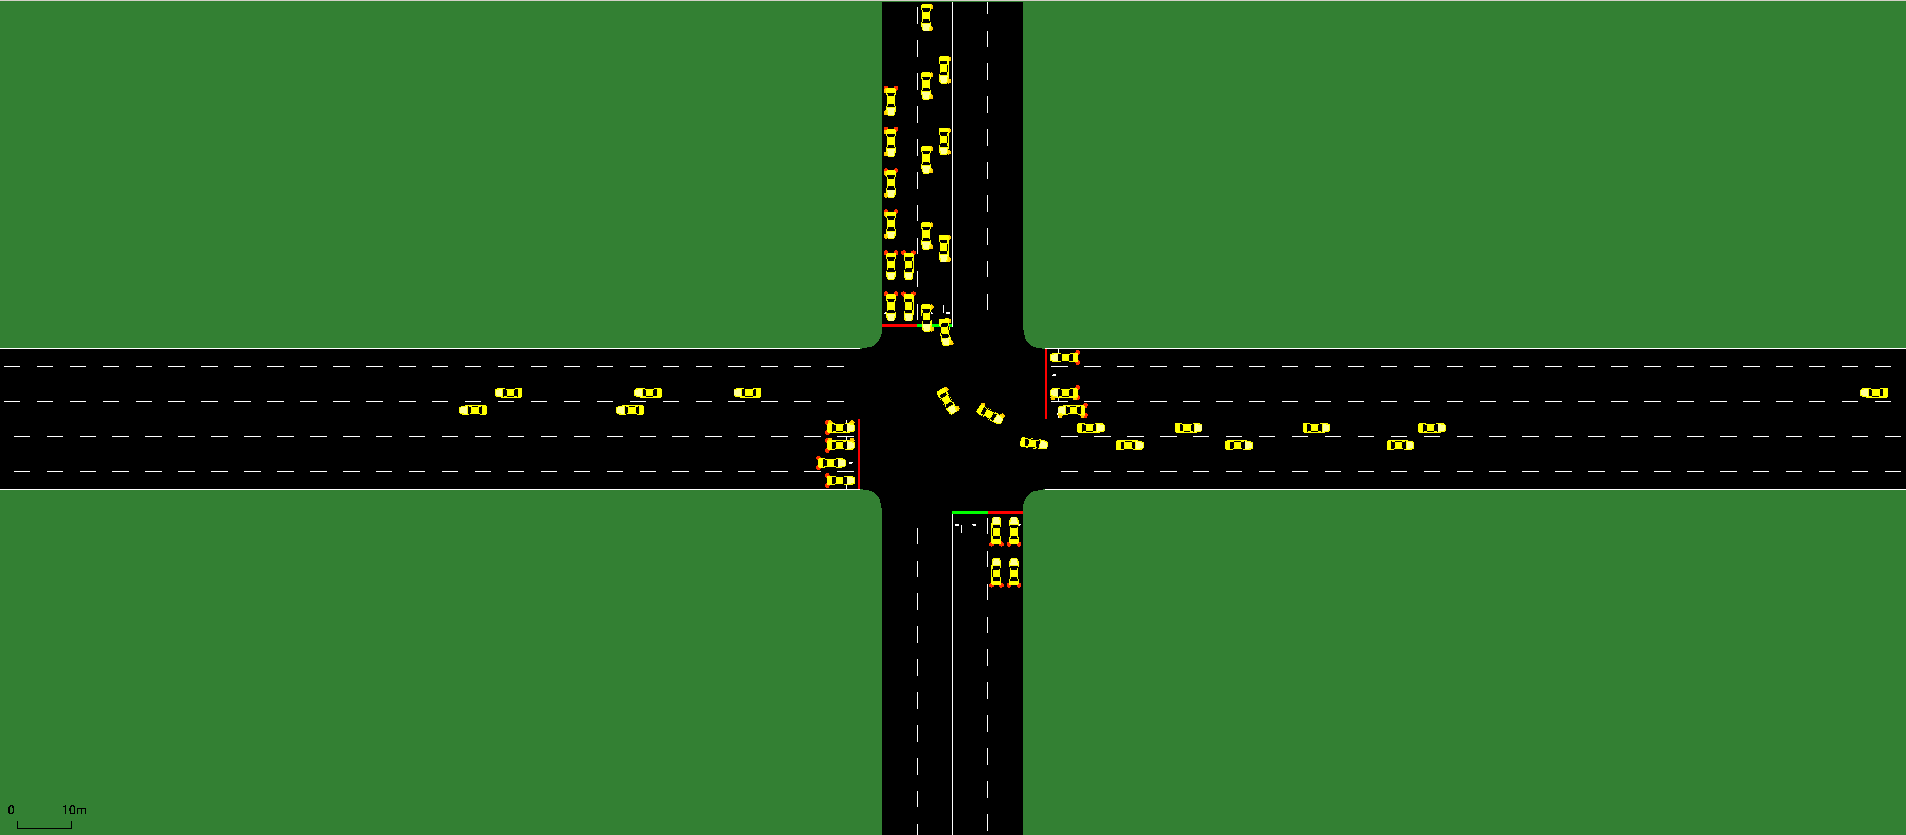
\includegraphics[width=\textwidth]{img/Appendix/scenario_c.png}
\centering
\end{figure}

\begin{figure}[h]
\subsubsection*{(d): 2 traffic lights, 4 phases, 3x3 incoming lanes.}
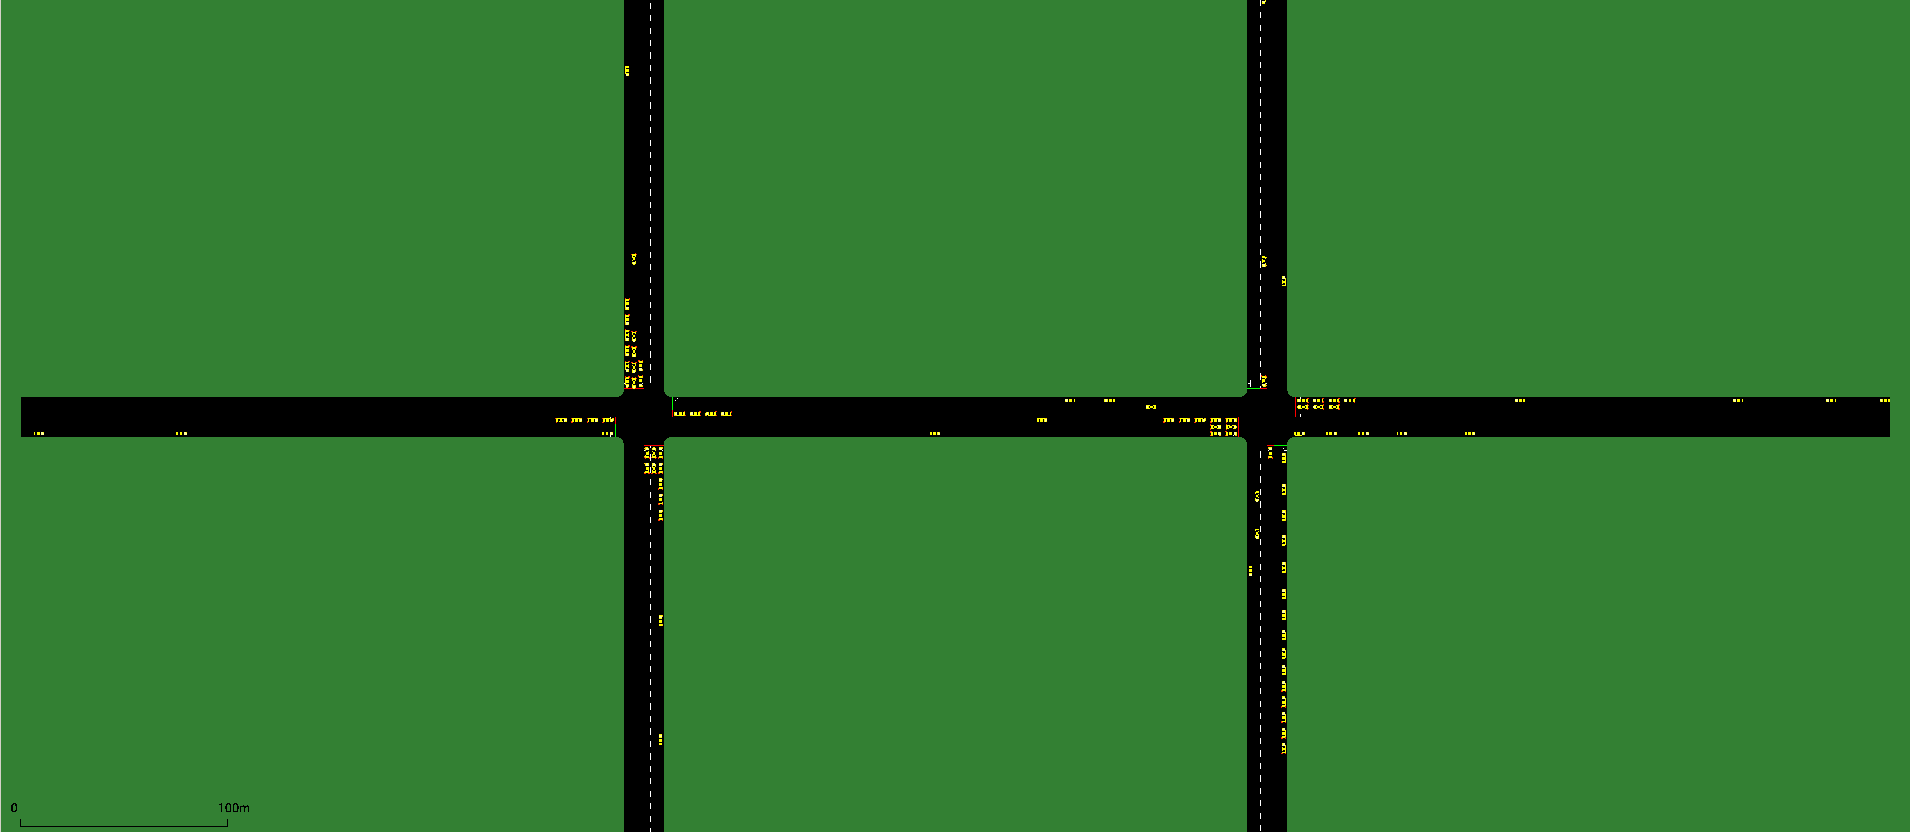
\includegraphics[width=\textwidth]{img/Appendix/scenario_d.png}
\centering
\end{figure}

\begin{figure}[h!]
\subsubsection*{(e): 4 traffic lights, 4 phases, 3x3 incoming lanes.}
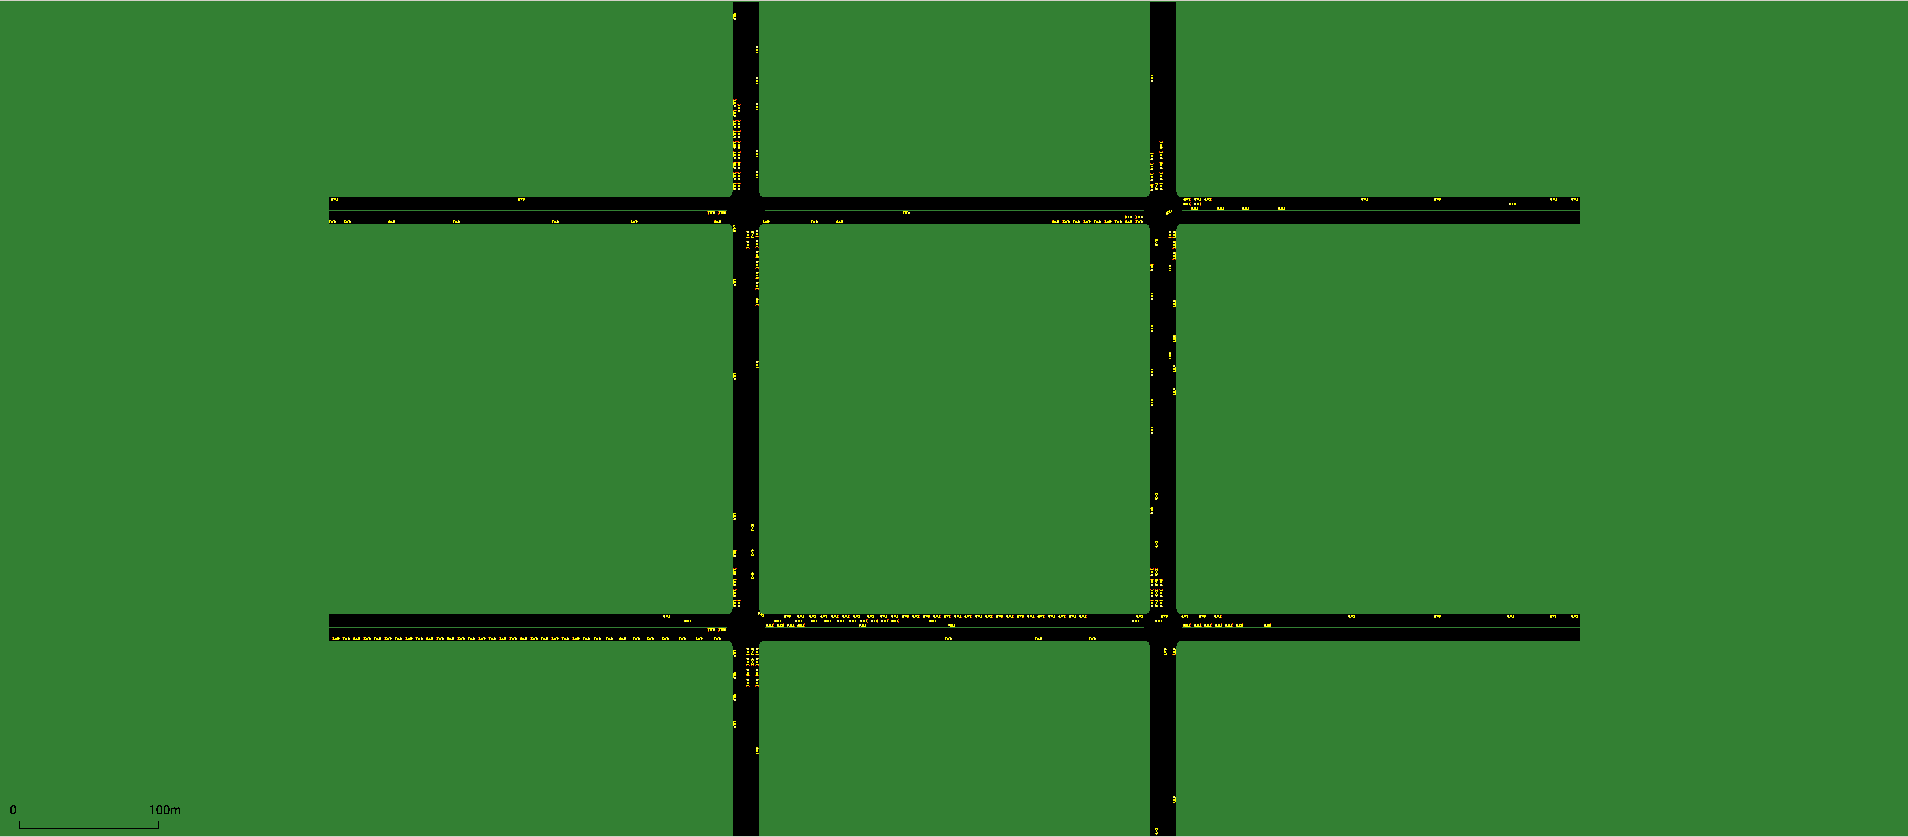
\includegraphics[width=\textwidth]{img/Appendix/scenario_e.png}
\centering
\end{figure}

\restoregeometry

\pagebreak

\subsection*{Appendix 2, Results (2.3.2) Analysis: figures, tables}
\addcontentsline{toc}{subsection}{Appendix 2, Results (2.3.2) Analysis: figures, tables}

This appendix contains the complete results for the DQN-ITSCwPD project, i.e. figures and tables, discussed in part 2.3.2.
Hereafter are the legends of following figures and tables: \\

\textbf{- 4 KP indicators:} \\
For all vehicles in all incoming lanes, the mean over one episode and the TLs of the total: 
\begin{enumerate}
    \setlength\itemsep{-0.5em}
    \item \textbf{Episode mean total accumulated waiting time}: accumulated waiting time;
    \item \textbf{Episode mean total delay}: delay;
    \item \textbf{Episode mean total queue length}: queue length;
    \item \textbf{Episode mean total volume}: volume.
\end{enumerate}

\textbf{- Traffic scenarios:} 
\begin{itemize}
    \setlength\itemsep{-0.5em}
    \item \textbf{(a)}: 1 traffic light, 2 phases, 2x2 incoming lanes;
    \item \textbf{(b)}: 1 traffic light, 4 phases, 3x3 incoming lanes;
    \item \textbf{(c)}: 1 traffic light, 4 phases, 4x4 incoming lanes;
    \item \textbf{(d)}: 2 traffic lights, 4 phases, 3x3 incoming lanes;
    \item \textbf{(e)}: 4 traffic lights, 4 phases, 3x3 incoming lanes.
\end{itemize}

\textbf{- Figure colors:}
\begin{itemize}
    \setlength\itemsep{-0.5em}
    \item \textbf{Blue}: DQN partial detection (DQN PD);
    \item \textbf{Orange}: DQN full detection (DQN FD);
    \item \textbf{Green}: Max Pressure full detection (MP FD);
    \item \textbf{Red}: SOTL full detection (SOTL FD);
    \item \textbf{Purple, brown, pink, grey, khaki}: scenarios (a), (b), (c), (d), (e).
\end{itemize}

\pagebreak

\newgeometry{left= 0.75cm, right= 0.75cm, bottom= 0cm, top= 0cm}
\begin{figure}[h]
\subsubsection*{(i, 1/3) Comparison of density distributions for full detection DQN, Max Pressure and SOTL; by 4 KPIs, and by scenario, and over 1000 episodes.}
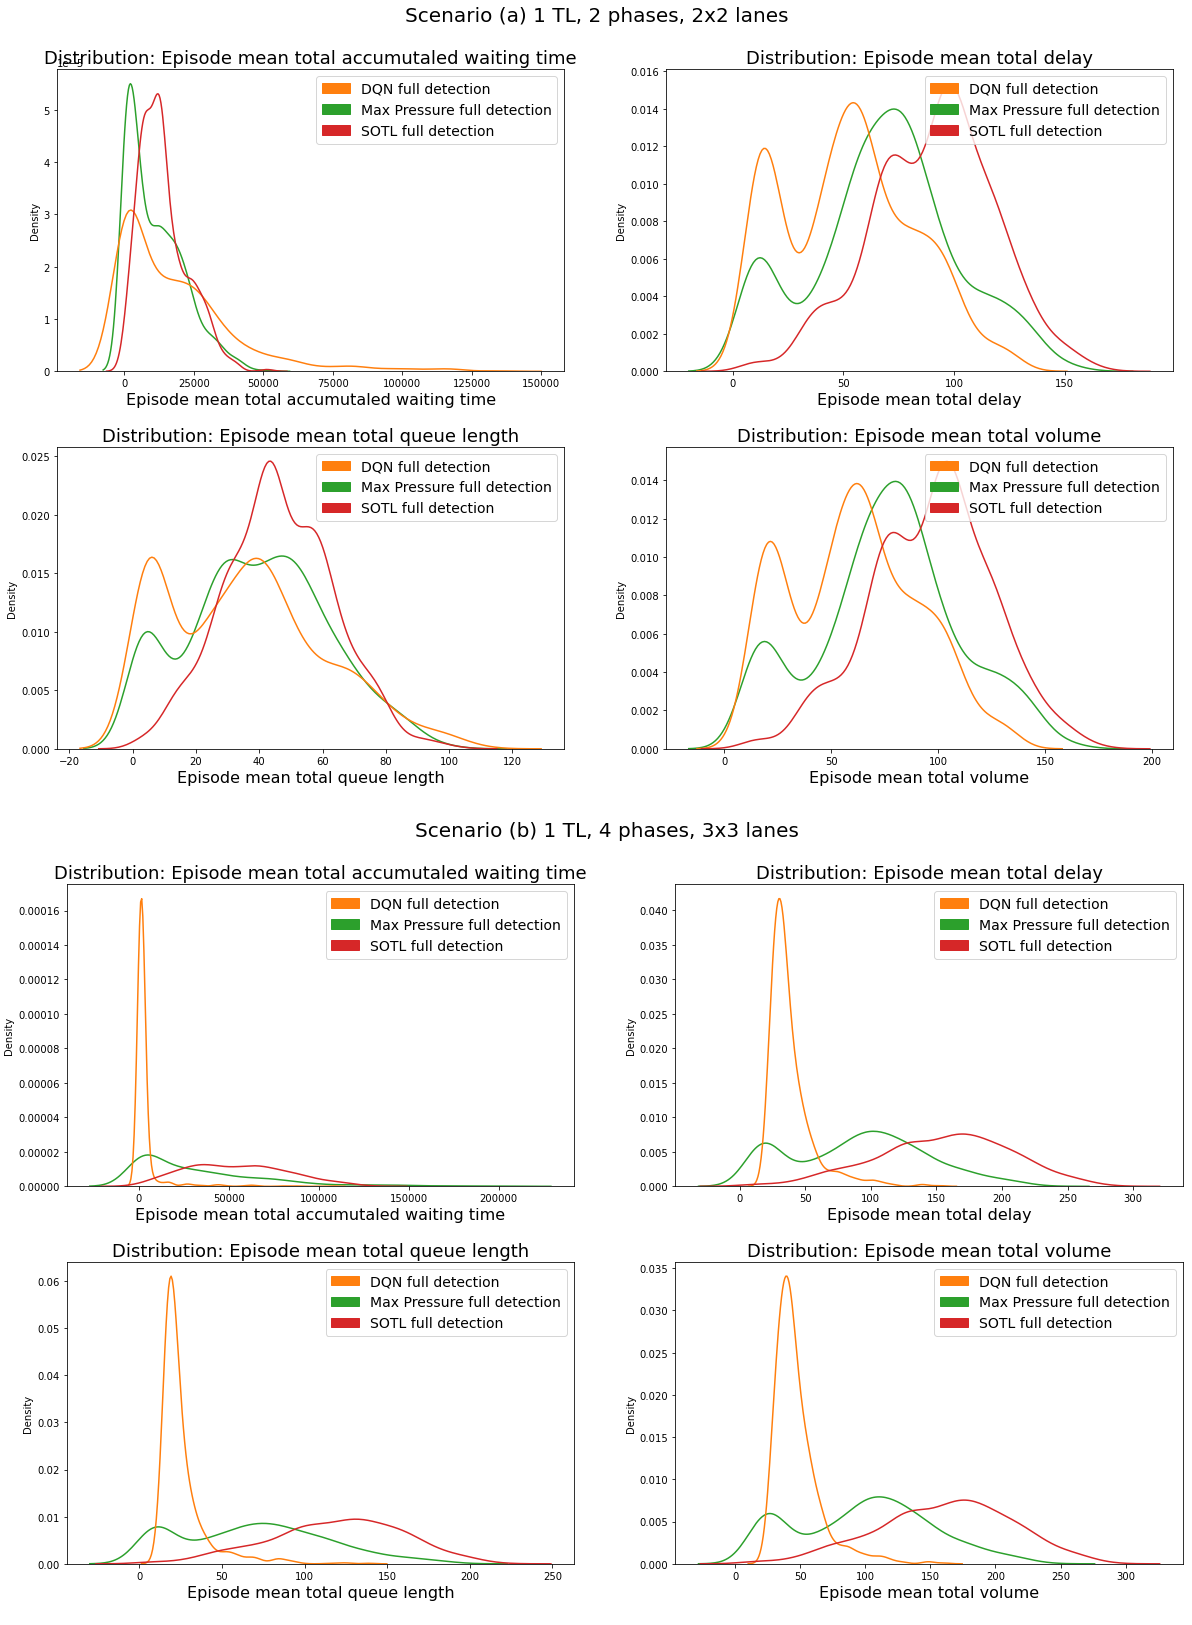
\includegraphics[width=\textwidth]{img/Appendix/1_1-2.png}
\centering
\end{figure}
\restoregeometry

\pagebreak

\newgeometry{left= 0.75cm, right= 0.75cm, bottom= 0cm, top= 0cm}
\begin{figure}[h]
\subsubsection*{(i, 2/3)}
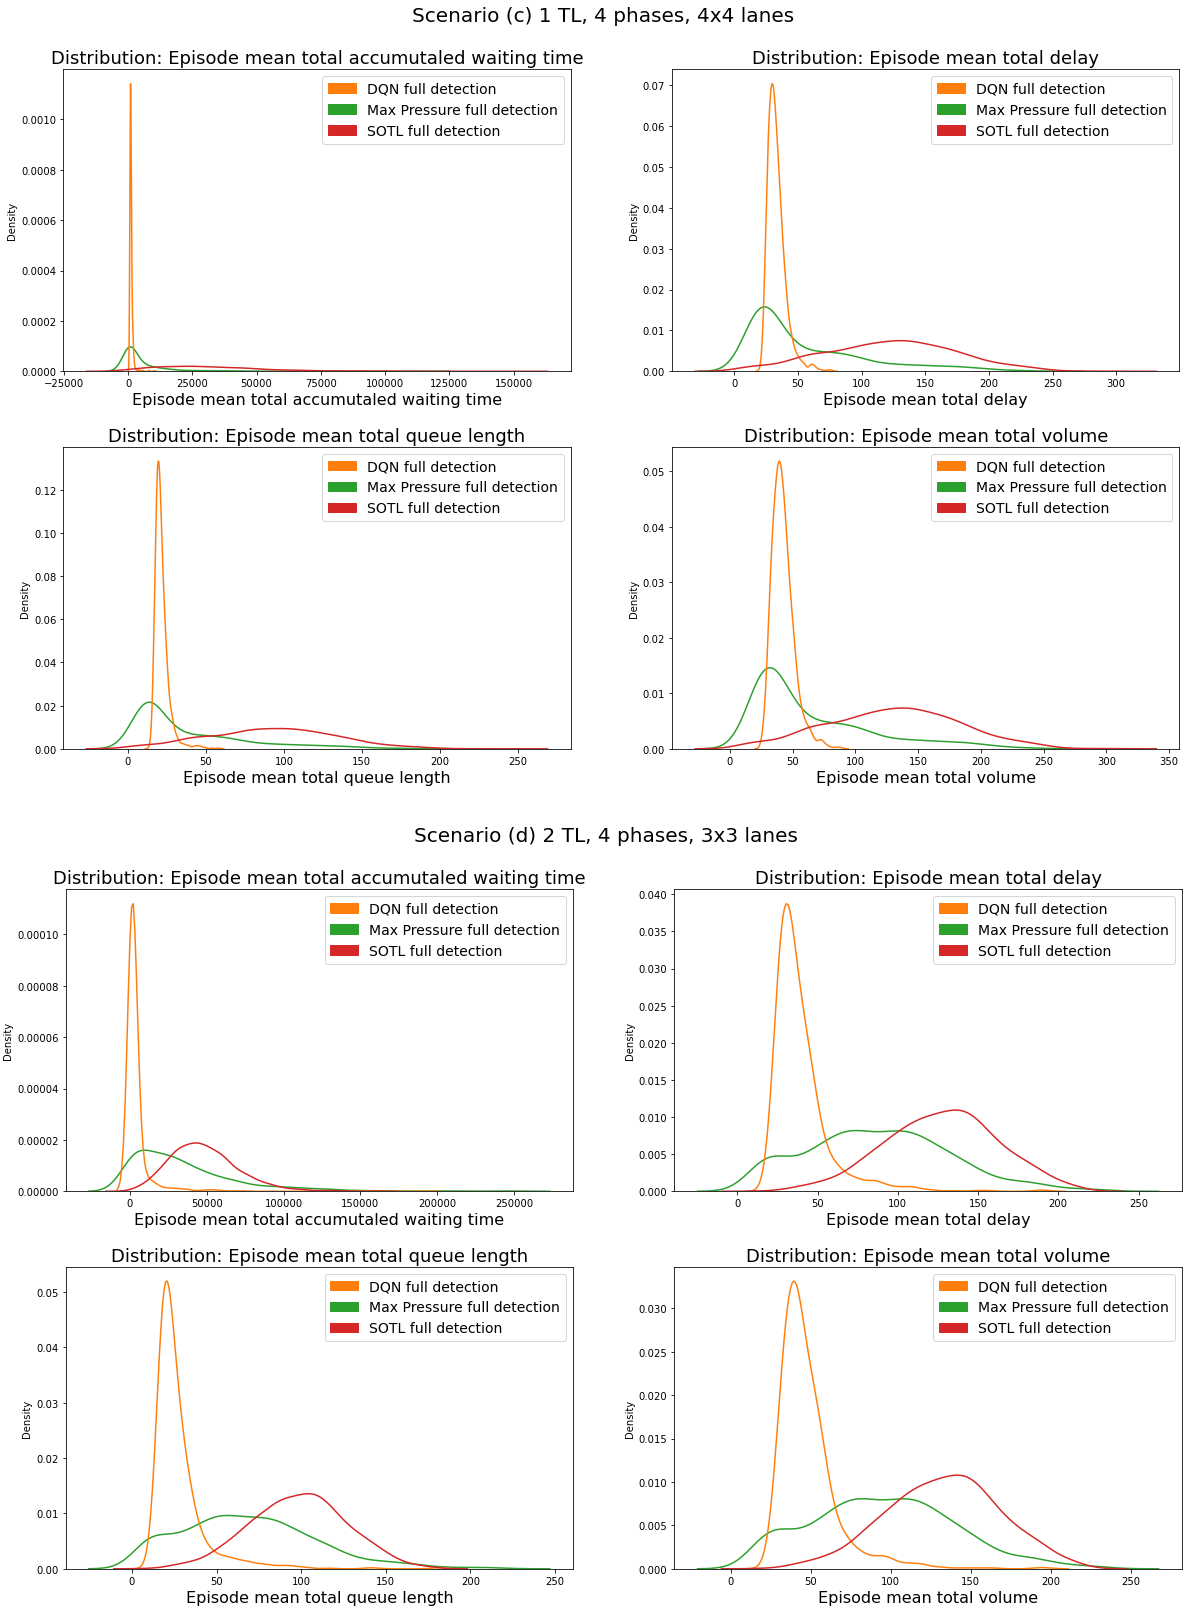
\includegraphics[width=\textwidth]{img/Appendix/1_3-4.png}
\centering
\end{figure}
\restoregeometry

\pagebreak

\newgeometry{left= 0.75cm, right= 0.75cm}
\begin{figure}[h]
\subsubsection*{(i, 3/3)}
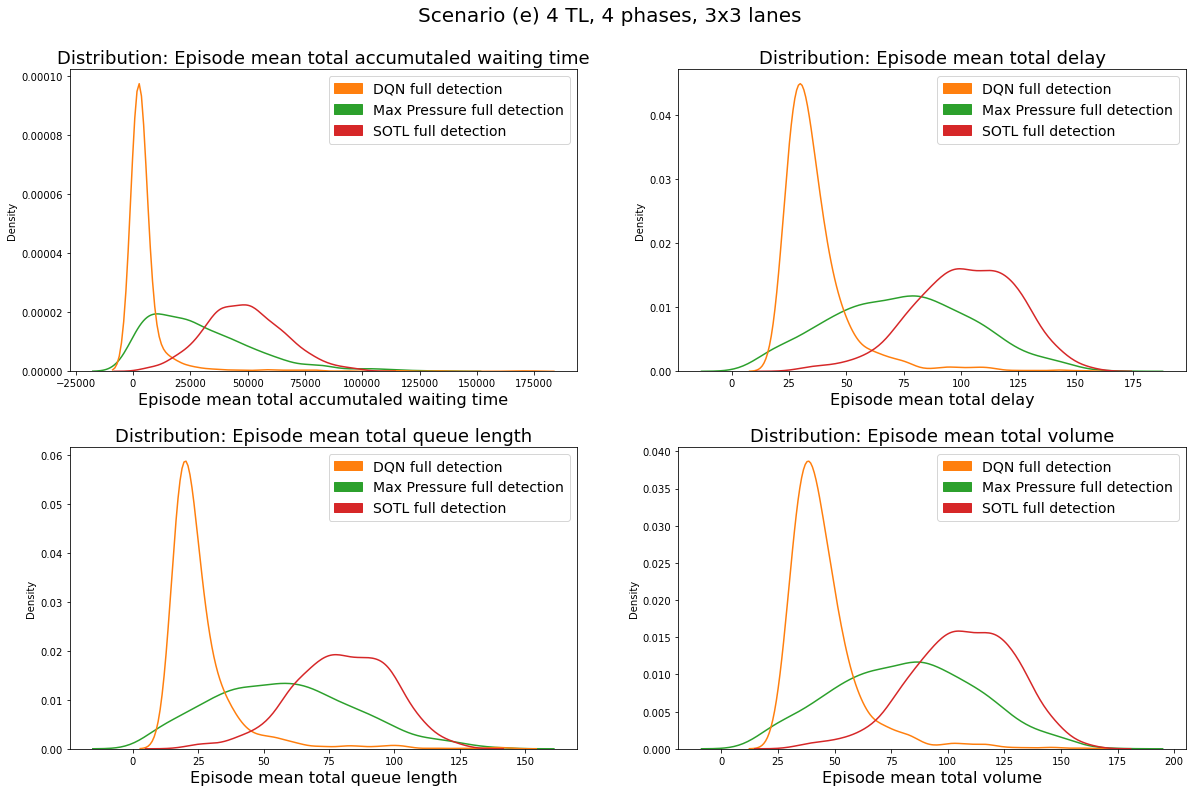
\includegraphics[width=\textwidth]{img/Appendix/1_5.png}
\centering
\end{figure}
\restoregeometry

\pagebreak

\newgeometry{left= 0.75cm, right= 0.75cm}
\begin{figure}[h]
\subsubsection*{(ii, 1/2) Comparison of statistics of 4 KPIs for full detection DQN, Max Pressure and SOTL; by scenario, and by mean, median, first quartile, third quartile, variance and standard deviation, and over 1000 episodes.}
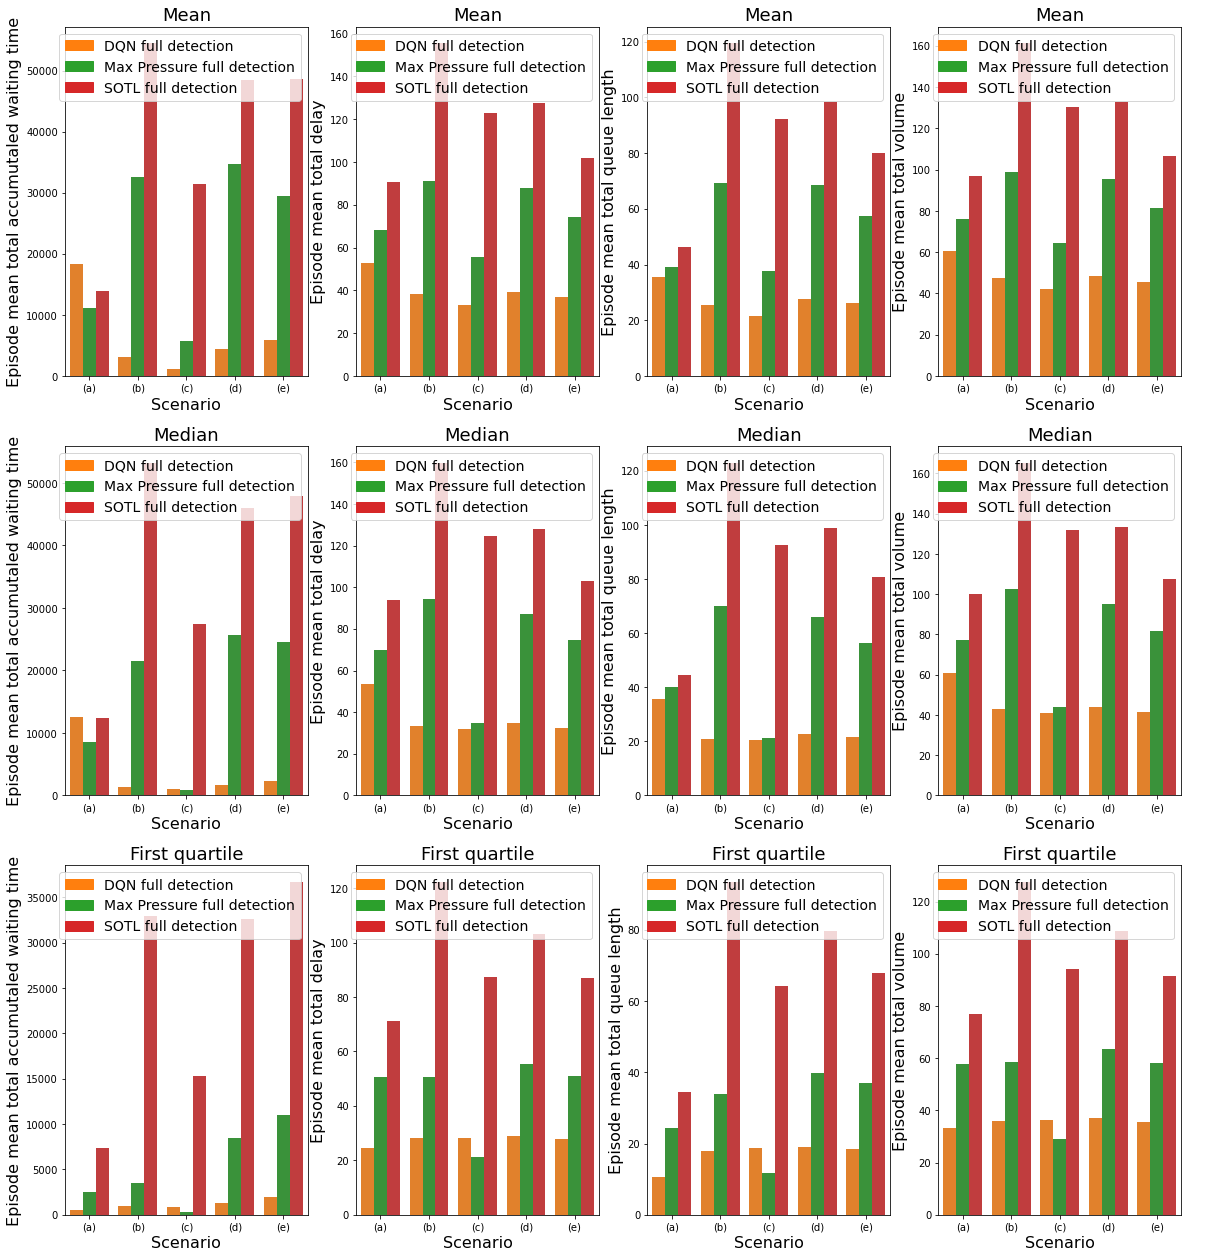
\includegraphics[width=\textwidth]{img/Appendix/2_1.png}
\centering
\end{figure}
\restoregeometry

\pagebreak

\newgeometry{left= 0.75cm, right= 0.75cm}
\begin{figure}[h]
\subsubsection*{(ii, 2/2)}
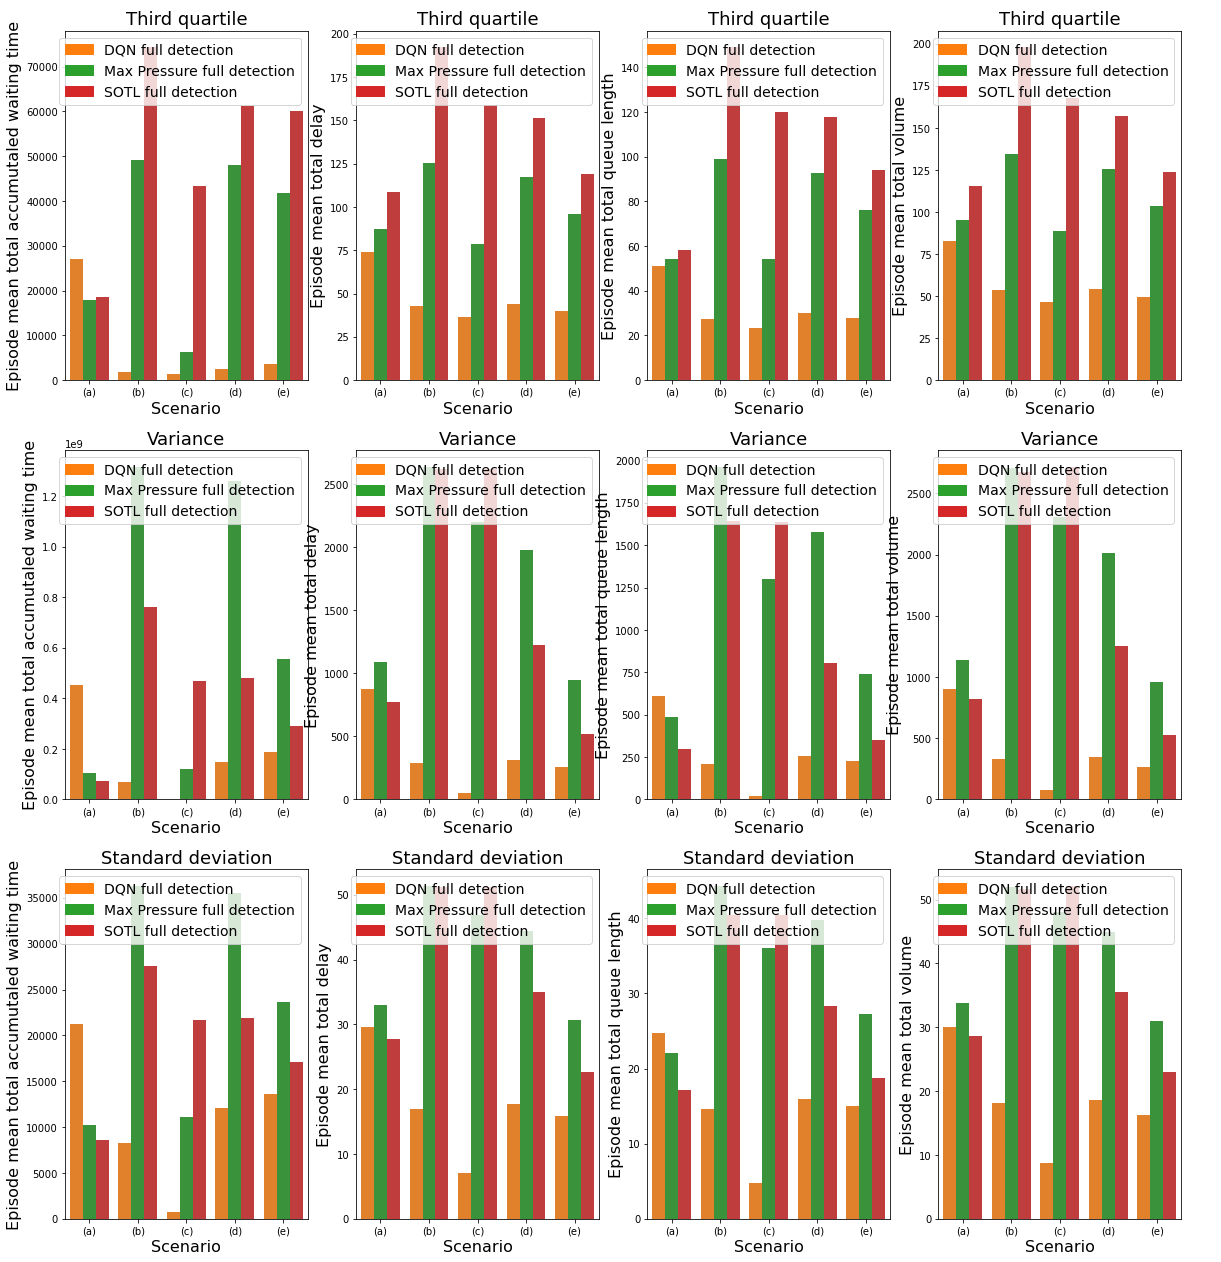
\includegraphics[width=\textwidth]{img/Appendix/2_2.png}
\centering
\end{figure}
\restoregeometry

\pagebreak

\newgeometry{left= 0.75cm, right= 0.75cm, bottom= 0cm, top= 0cm}
\begin{figure}[h]
\subsubsection*{(iii, 1/3) Comparison of 4 KPIs for full detection DQN and partial detection DQN; by penetration rate of connected vehicles, and by scenario, and over 1000 episodes.}
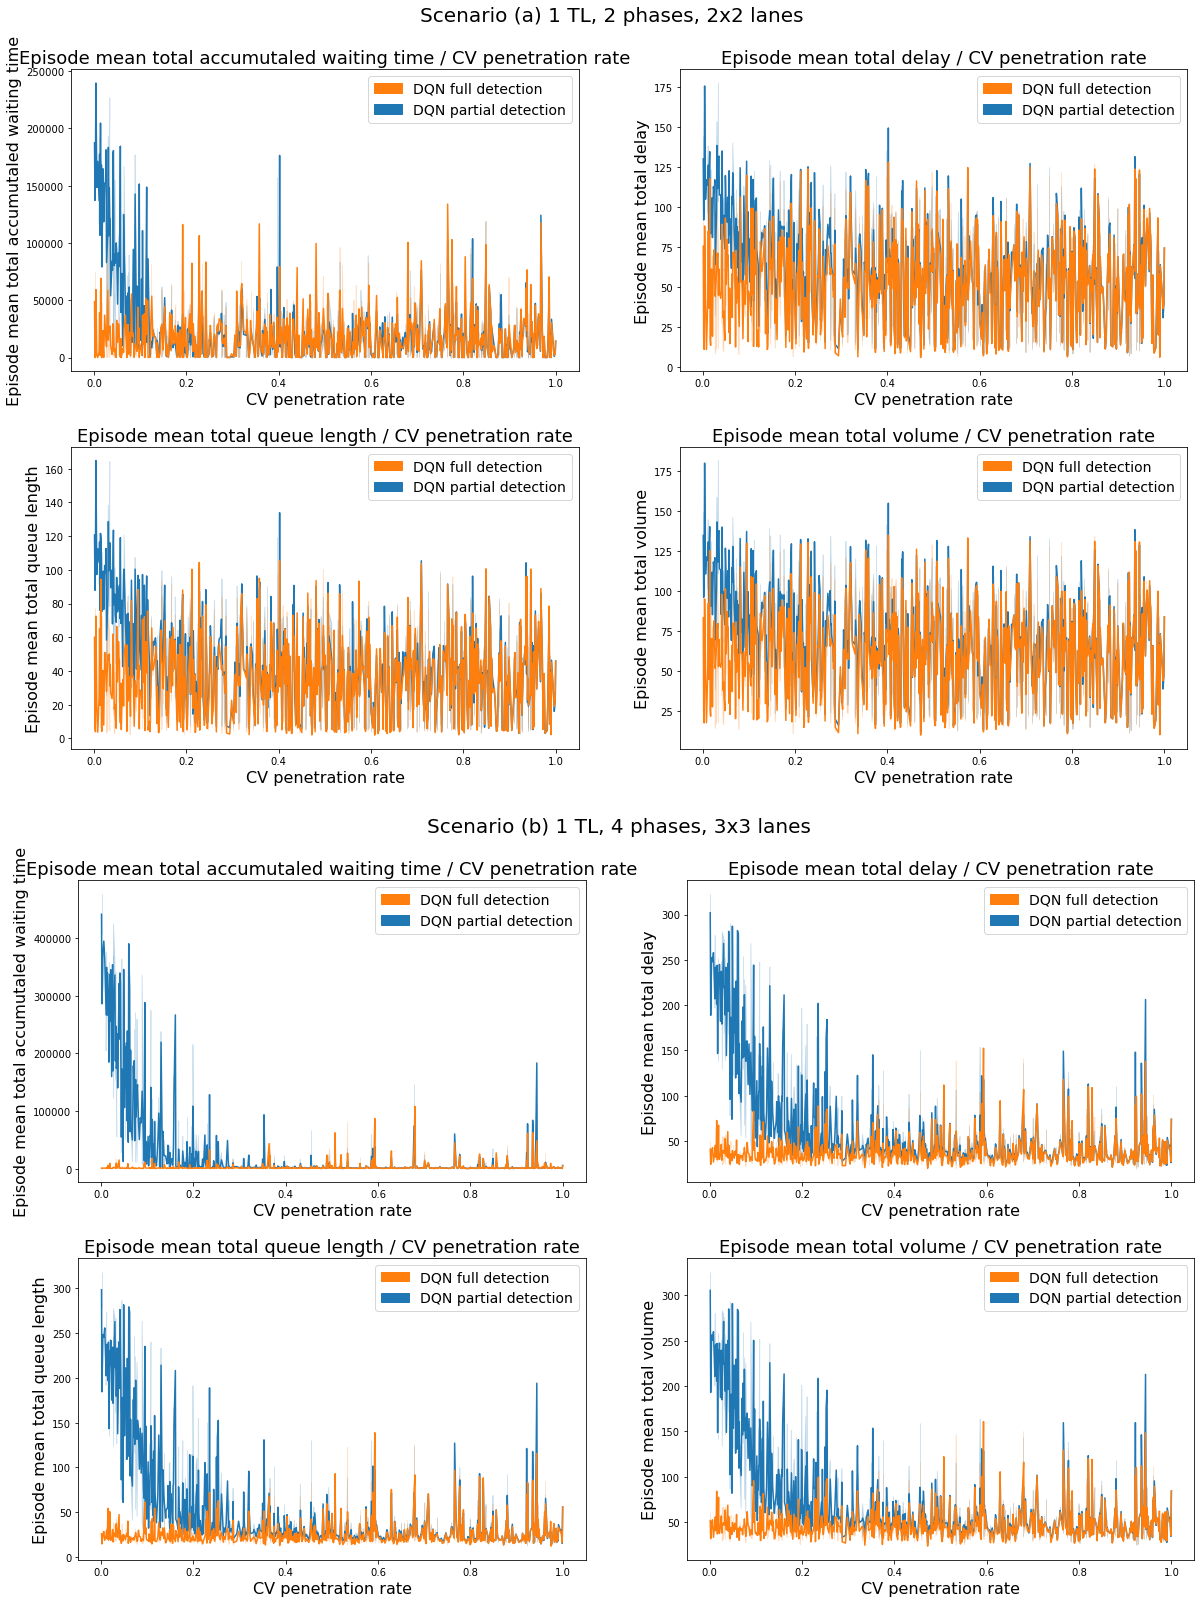
\includegraphics[width=\textwidth]{img/Appendix/3_1-2.png}
\centering
\end{figure}
\restoregeometry

\pagebreak

\newgeometry{left= 0.75cm, right= 0.75cm, bottom= 0cm, top= 0cm}
\begin{figure}[h]
\subsubsection*{(iii, 2/3)}
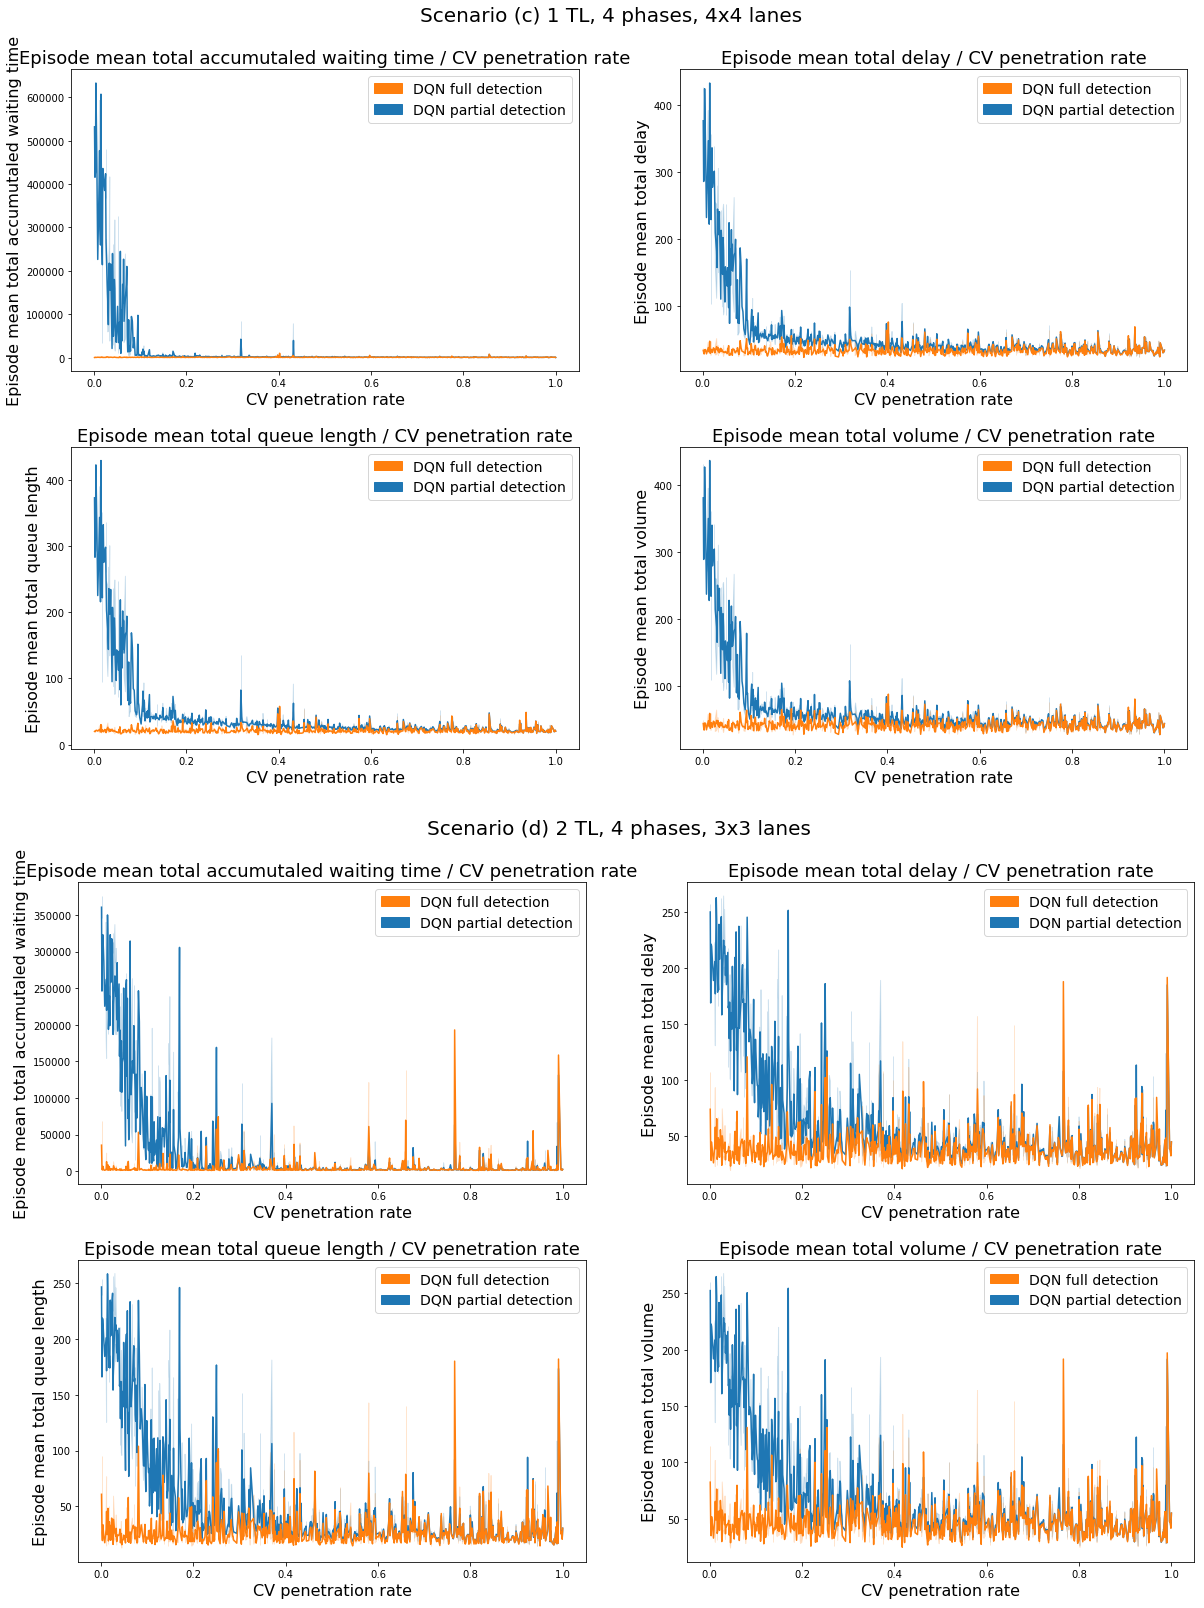
\includegraphics[width=\textwidth]{img/Appendix/3_3-4.png}
\centering
\end{figure}
\restoregeometry

\pagebreak

\newgeometry{left= 0.75cm, right= 0.75cm}
\begin{figure}[h]
\subsubsection*{(iii, 3/3)}
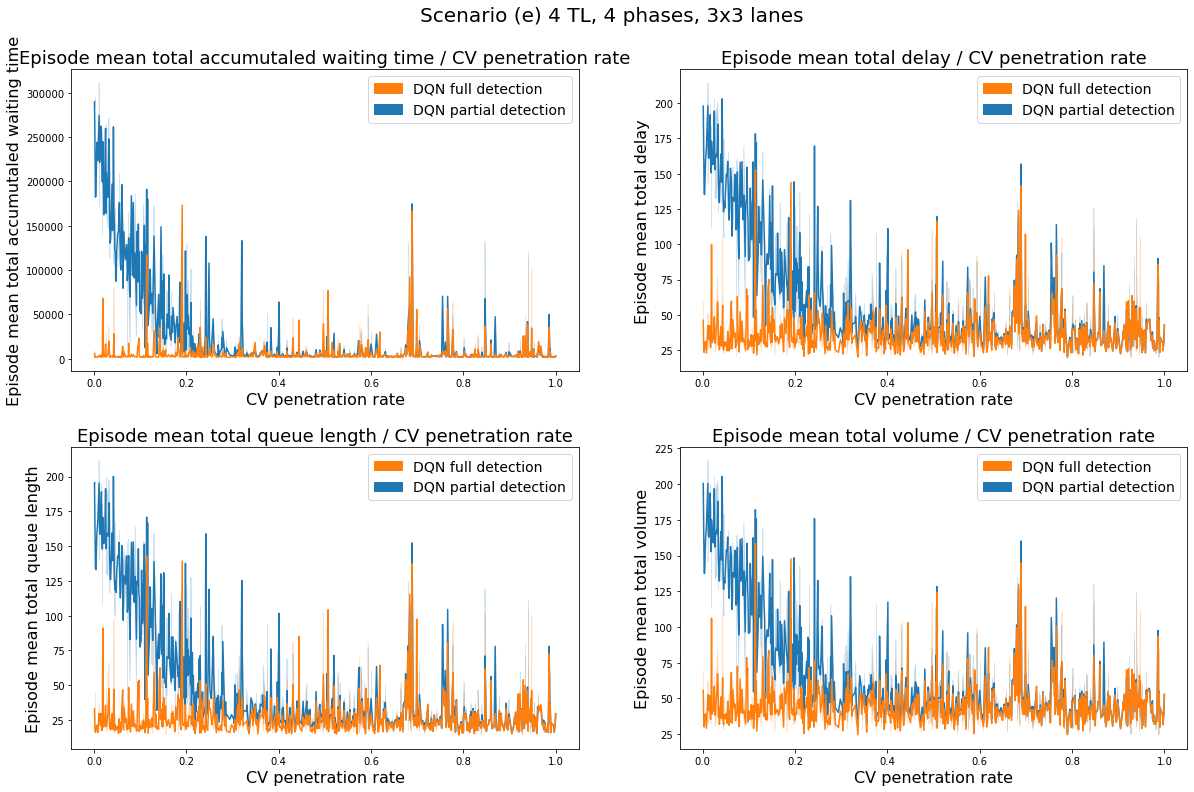
\includegraphics[width=\textwidth]{img/Appendix/3_5.png}
\centering
\end{figure}
\subsubsection*{(iv, 1/1) Comparison of percentage loss between full detection DQN and partial detection DQN of 4 KPIs for all scenarios; by range of penetration rates of connected vehicles, and over 1000 episodes.}
\restoregeometry

\pagebreak

\newgeometry{left= 0.75cm, right= 0.75cm, bottom= 0cm, top= 0cm}
\begin{figure}[h]
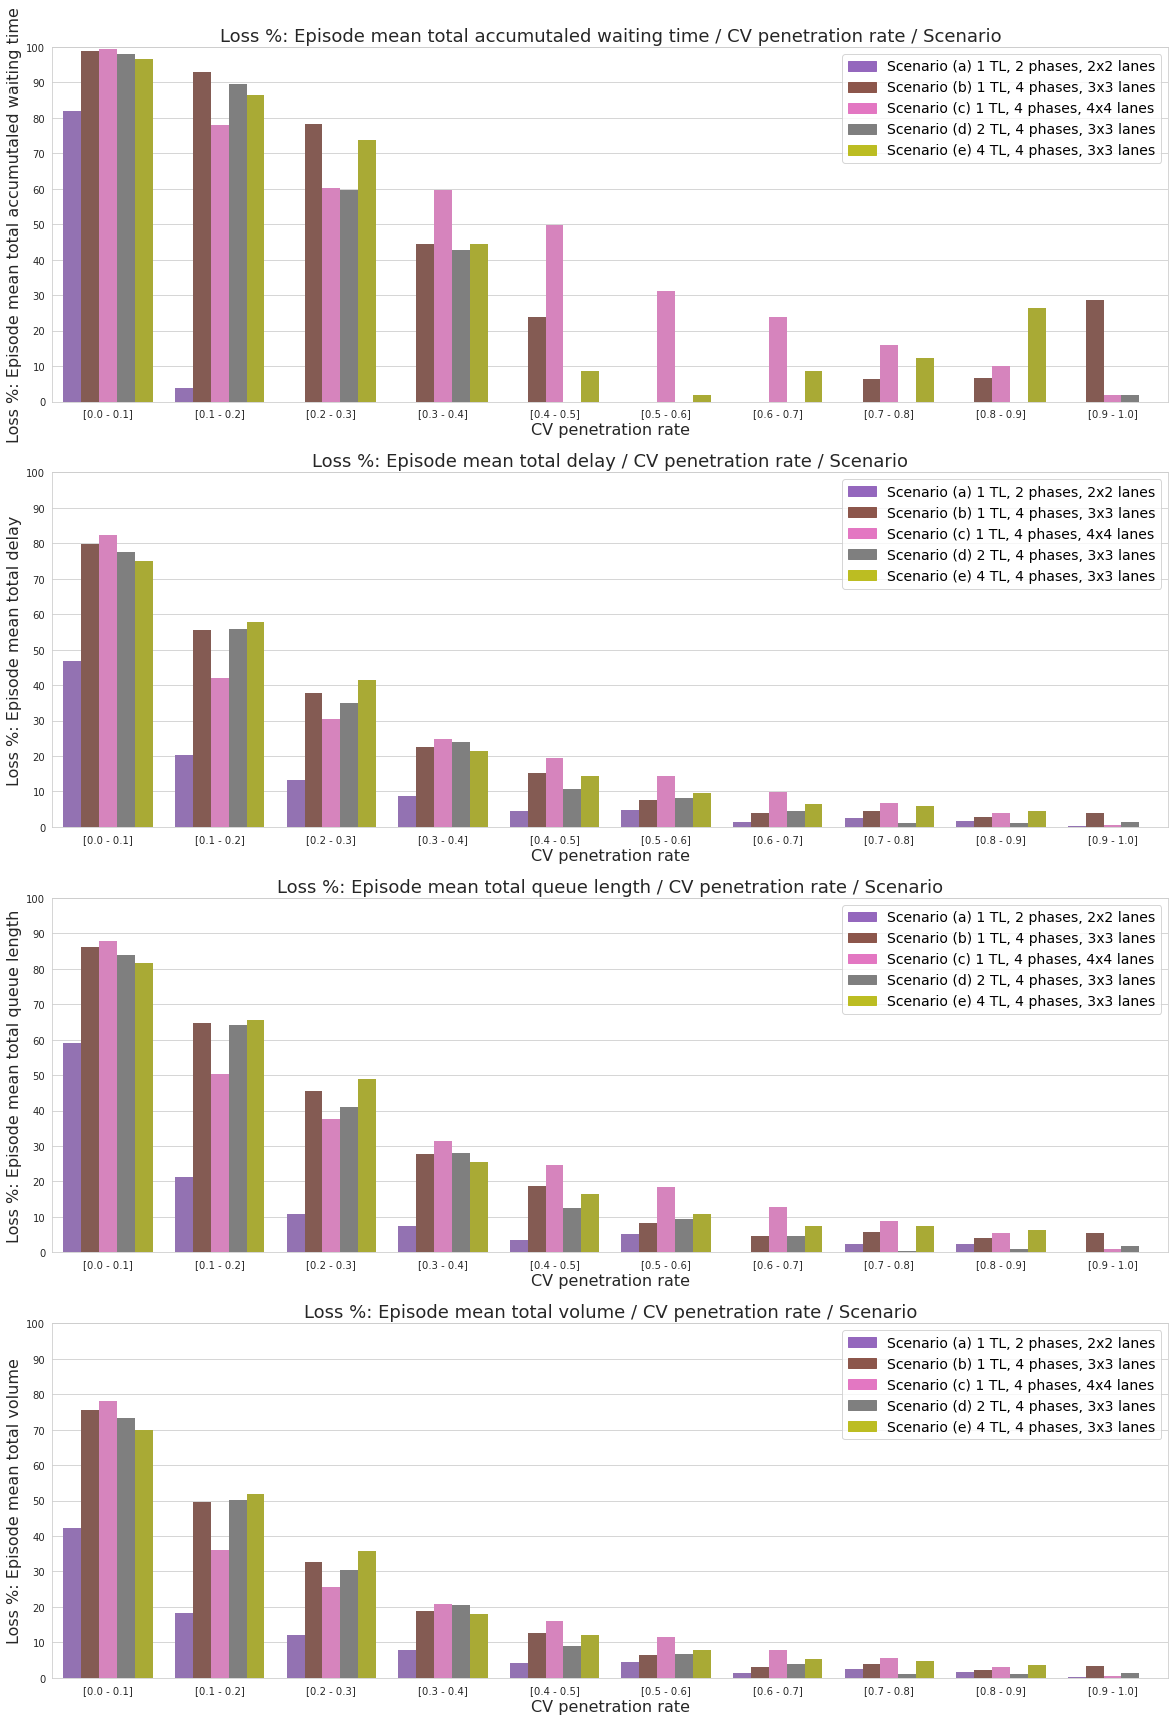
\includegraphics[width=\textwidth]{img/Appendix/4.png}
\centering
\end{figure}
\restoregeometry

\pagebreak

\subsubsection*{(v, 1/3) Table of numerical results for (ii). \\
(Comparison of statistics of 4 KPIs for full detection DQN, Max Pressure and SOTL; by scenario, and by mean, median, first quartile, third quartile, variance and standard deviation, and over 1000 episodes.)}

\begin{table}[htbp]
\centering
\setlength\tabcolsep{2pt}
\begin{tabular}{|c|c|}
\hline
Column &                                                           Title \\
\hline
     A &                                                        Scenario \\
     B &                                                       Algorithm \\
     C &               Mean: Episode mean total accumutaled waiting time \\
     D &                                  Mean: Episode mean total delay \\
     E &                           Mean: Episode mean total queue length \\
     F &                                 Mean: Episode mean total volume \\
     G &             Median: Episode mean total accumutaled waiting time \\
     H &                                Median: Episode mean total delay \\
     I &                         Median: Episode mean total queue length \\
     J &                               Median: Episode mean total volume \\
     K &     First quartile: Episode mean total accumutaled waiting time \\
     L &                        First quartile: Episode mean total delay \\
     M &                 First quartile: Episode mean total queue length \\
     N &                       First quartile: Episode mean total volume \\
     O &     Third quartile: Episode mean total accumutaled waiting time \\
     P &                        Third quartile: Episode mean total delay \\
     Q &                 Third quartile: Episode mean total queue length \\
     R &                       Third quartile: Episode mean total volume \\
     S &           Variance: Episode mean total accumutaled waiting time \\
     T &                              Variance: Episode mean total delay \\
     U &                       Variance: Episode mean total queue length \\
     V &                             Variance: Episode mean total volume \\
     W & Standard deviation: Episode mean total accumutaled waiting time \\
     X &                    Standard deviation: Episode mean total delay \\
     Y &             Standard deviation: Episode mean total queue length \\
     Z &                   Standard deviation: Episode mean total volume \\
\hline
\end{tabular}
\end{table}

\pagebreak

\newgeometry{left= 0cm, right= 0cm, bottom= 0cm, top= 0cm}

\begin{table}[htbp]
\centering
\small
\setlength\tabcolsep{2pt}
\begin{tabular}{|c|c|c|c|c|c|c|c|c|c|c|c|c|c|}
\hline
{} &    A &          B &       C &     D &     E &     F &       G &     H &     I &     J &       K &     L &    M \\
\hline
0  &  (a) &   DQN (FD) & 18280.2 &  52.8 &  35.7 &  60.6 & 12542.0 &  53.3 &  35.7 &  61.1 &   475.1 &  24.6 & 10.6 \\
1  &  (a) &    MP (FD) & 11130.9 &  68.1 &  39.3 &  76.0 &  8528.5 &  69.8 &  40.0 &  77.4 &  2543.0 &  50.4 & 24.5 \\
2  &  (a) &  SOTL (FD) & 13864.7 &  90.5 &  46.2 &  96.8 & 12433.5 &  94.0 &  44.6 & 100.0 &  7325.2 &  71.3 & 34.4 \\
3  &  (a) &   DQN (FD) & 18280.2 &  52.8 &  35.7 &  60.6 & 12542.0 &  53.3 &  35.7 &  61.1 &   475.1 &  24.6 & 10.6 \\
4  &  (a) &    MP (FD) & 11130.9 &  68.1 &  39.3 &  76.0 &  8528.5 &  69.8 &  40.0 &  77.4 &  2543.0 &  50.4 & 24.5 \\
5  &  (a) &  SOTL (FD) & 13864.7 &  90.5 &  46.2 &  96.8 & 12433.5 &  94.0 &  44.6 & 100.0 &  7325.2 &  71.3 & 34.4 \\
6  &  (a) &   DQN (FD) & 18280.2 &  52.8 &  35.7 &  60.6 & 12542.0 &  53.3 &  35.7 &  61.1 &   475.1 &  24.6 & 10.6 \\
7  &  (a) &    MP (FD) & 11130.9 &  68.1 &  39.3 &  76.0 &  8528.5 &  69.8 &  40.0 &  77.4 &  2543.0 &  50.4 & 24.5 \\
8  &  (a) &  SOTL (FD) & 13864.7 &  90.5 &  46.2 &  96.8 & 12433.5 &  94.0 &  44.6 & 100.0 &  7325.2 &  71.3 & 34.4 \\
9  &  (a) &   DQN (FD) & 18280.2 &  52.8 &  35.7 &  60.6 & 12542.0 &  53.3 &  35.7 &  61.1 &   475.1 &  24.6 & 10.6 \\
10 &  (a) &    MP (FD) & 11130.9 &  68.1 &  39.3 &  76.0 &  8528.5 &  69.8 &  40.0 &  77.4 &  2543.0 &  50.4 & 24.5 \\
11 &  (a) &  SOTL (FD) & 13864.7 &  90.5 &  46.2 &  96.8 & 12433.5 &  94.0 &  44.6 & 100.0 &  7325.2 &  71.3 & 34.4 \\
12 &  (b) &   DQN (FD) &  3127.5 &  38.4 &  25.7 &  47.5 &  1276.8 &  33.2 &  20.8 &  42.8 &   997.1 &  28.2 & 17.8 \\
13 &  (b) &    MP (FD) & 32511.5 &  90.9 &  69.3 &  99.1 & 21531.7 &  94.4 &  69.9 & 102.6 &  3533.2 &  50.5 & 33.8 \\
14 &  (b) &  SOTL (FD) & 54466.6 & 155.5 & 119.4 & 161.3 & 53266.0 & 159.9 & 123.1 & 165.4 & 32988.7 & 122.3 & 93.4 \\
15 &  (b) &   DQN (FD) &  3127.5 &  38.4 &  25.7 &  47.5 &  1276.8 &  33.2 &  20.8 &  42.8 &   997.1 &  28.2 & 17.8 \\
16 &  (b) &    MP (FD) & 32511.5 &  90.9 &  69.3 &  99.1 & 21531.7 &  94.4 &  69.9 & 102.6 &  3533.2 &  50.5 & 33.8 \\
17 &  (b) &  SOTL (FD) & 54466.6 & 155.5 & 119.4 & 161.3 & 53266.0 & 159.9 & 123.1 & 165.4 & 32988.7 & 122.3 & 93.4 \\
18 &  (b) &   DQN (FD) &  3127.5 &  38.4 &  25.7 &  47.5 &  1276.8 &  33.2 &  20.8 &  42.8 &   997.1 &  28.2 & 17.8 \\
19 &  (b) &    MP (FD) & 32511.5 &  90.9 &  69.3 &  99.1 & 21531.7 &  94.4 &  69.9 & 102.6 &  3533.2 &  50.5 & 33.8 \\
20 &  (b) &  SOTL (FD) & 54466.6 & 155.5 & 119.4 & 161.3 & 53266.0 & 159.9 & 123.1 & 165.4 & 32988.7 & 122.3 & 93.4 \\
21 &  (b) &   DQN (FD) &  3127.5 &  38.4 &  25.7 &  47.5 &  1276.8 &  33.2 &  20.8 &  42.8 &   997.1 &  28.2 & 17.8 \\
22 &  (b) &    MP (FD) & 32511.5 &  90.9 &  69.3 &  99.1 & 21531.7 &  94.4 &  69.9 & 102.6 &  3533.2 &  50.5 & 33.8 \\
23 &  (b) &  SOTL (FD) & 54466.6 & 155.5 & 119.4 & 161.3 & 53266.0 & 159.9 & 123.1 & 165.4 & 32988.7 & 122.3 & 93.4 \\
24 &  (c) &   DQN (FD) &  1165.9 &  33.2 &  21.6 &  42.3 &  1017.9 &  31.7 &  20.5 &  40.9 &   840.3 &  28.2 & 18.8 \\
25 &  (c) &    MP (FD) &  5726.8 &  55.5 &  37.7 &  64.3 &   824.4 &  34.7 &  21.2 &  44.0 &   302.0 &  21.3 & 11.8 \\
26 &  (c) &  SOTL (FD) & 31387.7 & 122.7 &  92.2 & 130.2 & 27506.7 & 124.8 &  92.7 & 132.0 & 15308.8 &  87.3 & 64.1 \\
27 &  (c) &   DQN (FD) &  1165.9 &  33.2 &  21.6 &  42.3 &  1017.9 &  31.7 &  20.5 &  40.9 &   840.3 &  28.2 & 18.8 \\
28 &  (c) &    MP (FD) &  5726.8 &  55.5 &  37.7 &  64.3 &   824.4 &  34.7 &  21.2 &  44.0 &   302.0 &  21.3 & 11.8 \\
29 &  (c) &  SOTL (FD) & 31387.7 & 122.7 &  92.2 & 130.2 & 27506.7 & 124.8 &  92.7 & 132.0 & 15308.8 &  87.3 & 64.1 \\
30 &  (c) &   DQN (FD) &  1165.9 &  33.2 &  21.6 &  42.3 &  1017.9 &  31.7 &  20.5 &  40.9 &   840.3 &  28.2 & 18.8 \\
31 &  (c) &    MP (FD) &  5726.8 &  55.5 &  37.7 &  64.3 &   824.4 &  34.7 &  21.2 &  44.0 &   302.0 &  21.3 & 11.8 \\
32 &  (c) &  SOTL (FD) & 31387.7 & 122.7 &  92.2 & 130.2 & 27506.7 & 124.8 &  92.7 & 132.0 & 15308.8 &  87.3 & 64.1 \\
33 &  (c) &   DQN (FD) &  1165.9 &  33.2 &  21.6 &  42.3 &  1017.9 &  31.7 &  20.5 &  40.9 &   840.3 &  28.2 & 18.8 \\
34 &  (c) &    MP (FD) &  5726.8 &  55.5 &  37.7 &  64.3 &   824.4 &  34.7 &  21.2 &  44.0 &   302.0 &  21.3 & 11.8 \\
35 &  (c) &  SOTL (FD) & 31387.7 & 122.7 &  92.2 & 130.2 & 27506.7 & 124.8 &  92.7 & 132.0 & 15308.8 &  87.3 & 64.1 \\
36 &  (d) &   DQN (FD) &  4369.0 &  39.4 &  27.6 &  48.3 &  1659.8 &  34.5 &  22.8 &  43.7 &  1318.2 &  28.9 & 19.0 \\
37 &  (d) &    MP (FD) & 34699.3 &  87.8 &  68.6 &  95.4 & 25703.6 &  87.0 &  66.0 &  95.0 &  8458.1 &  55.5 & 39.7 \\
38 &  (d) &  SOTL (FD) & 48387.8 & 127.5 &  98.5 & 133.0 & 45930.0 & 128.1 &  99.0 & 133.4 & 32574.7 & 103.2 & 79.7 \\
39 &  (d) &   DQN (FD) &  4369.0 &  39.4 &  27.6 &  48.3 &  1659.8 &  34.5 &  22.8 &  43.7 &  1318.2 &  28.9 & 19.0 \\
40 &  (d) &    MP (FD) & 34699.3 &  87.8 &  68.6 &  95.4 & 25703.6 &  87.0 &  66.0 &  95.0 &  8458.1 &  55.5 & 39.7 \\
41 &  (d) &  SOTL (FD) & 48387.8 & 127.5 &  98.5 & 133.0 & 45930.0 & 128.1 &  99.0 & 133.4 & 32574.7 & 103.2 & 79.7 \\
42 &  (d) &   DQN (FD) &  4369.0 &  39.4 &  27.6 &  48.3 &  1659.8 &  34.5 &  22.8 &  43.7 &  1318.2 &  28.9 & 19.0 \\
43 &  (d) &    MP (FD) & 34699.3 &  87.8 &  68.6 &  95.4 & 25703.6 &  87.0 &  66.0 &  95.0 &  8458.1 &  55.5 & 39.7 \\
44 &  (d) &  SOTL (FD) & 48387.8 & 127.5 &  98.5 & 133.0 & 45930.0 & 128.1 &  99.0 & 133.4 & 32574.7 & 103.2 & 79.7 \\
45 &  (d) &   DQN (FD) &  4369.0 &  39.4 &  27.6 &  48.3 &  1659.8 &  34.5 &  22.8 &  43.7 &  1318.2 &  28.9 & 19.0 \\
46 &  (d) &    MP (FD) & 34699.3 &  87.8 &  68.6 &  95.4 & 25703.6 &  87.0 &  66.0 &  95.0 &  8458.1 &  55.5 & 39.7 \\
47 &  (d) &  SOTL (FD) & 48387.8 & 127.5 &  98.5 & 133.0 & 45930.0 & 128.1 &  99.0 & 133.4 & 32574.7 & 103.2 & 79.7 \\
48 &  (e) &   DQN (FD) &  5867.3 &  36.9 &  26.2 &  45.4 &  2385.1 &  32.5 &  21.8 &  41.4 &  1966.9 &  27.7 & 18.4 \\
49 &  (e) &    MP (FD) & 29462.5 &  74.4 &  57.5 &  81.6 & 24554.7 &  74.8 &  56.3 &  81.8 & 10953.9 &  50.9 & 37.0 \\
50 &  (e) &  SOTL (FD) & 48573.9 & 102.0 &  80.1 & 106.8 & 47873.2 & 102.9 &  80.7 & 107.8 & 36692.6 &  86.9 & 67.7 \\
51 &  (e) &   DQN (FD) &  5867.3 &  36.9 &  26.2 &  45.4 &  2385.1 &  32.5 &  21.8 &  41.4 &  1966.9 &  27.7 & 18.4 \\
52 &  (e) &    MP (FD) & 29462.5 &  74.4 &  57.5 &  81.6 & 24554.7 &  74.8 &  56.3 &  81.8 & 10953.9 &  50.9 & 37.0 \\
53 &  (e) &  SOTL (FD) & 48573.9 & 102.0 &  80.1 & 106.8 & 47873.2 & 102.9 &  80.7 & 107.8 & 36692.6 &  86.9 & 67.7 \\
54 &  (e) &   DQN (FD) &  5867.3 &  36.9 &  26.2 &  45.4 &  2385.1 &  32.5 &  21.8 &  41.4 &  1966.9 &  27.7 & 18.4 \\
55 &  (e) &    MP (FD) & 29462.5 &  74.4 &  57.5 &  81.6 & 24554.7 &  74.8 &  56.3 &  81.8 & 10953.9 &  50.9 & 37.0 \\
56 &  (e) &  SOTL (FD) & 48573.9 & 102.0 &  80.1 & 106.8 & 47873.2 & 102.9 &  80.7 & 107.8 & 36692.6 &  86.9 & 67.7 \\
57 &  (e) &   DQN (FD) &  5867.3 &  36.9 &  26.2 &  45.4 &  2385.1 &  32.5 &  21.8 &  41.4 &  1966.9 &  27.7 & 18.4 \\
58 &  (e) &    MP (FD) & 29462.5 &  74.4 &  57.5 &  81.6 & 24554.7 &  74.8 &  56.3 &  81.8 & 10953.9 &  50.9 & 37.0 \\
59 &  (e) &  SOTL (FD) & 48573.9 & 102.0 &  80.1 & 106.8 & 47873.2 & 102.9 &  80.7 & 107.8 & 36692.6 &  86.9 & 67.7 \\
\hline
\end{tabular}
\end{table}

\pagebreak

\begin{table}[htbp]
\centering
\small
\setlength\tabcolsep{2pt}
\begin{tabular}{|c|c|c|c|c|c|c|c|c|c|c|c|c|c|}
\hline
{} &     N &       O &     P &     Q &     R &            S &      T &      U &      V &       W &    X &    Y &    Z \\
\hline
0  &  33.4 & 27001.3 &  74.0 &  50.9 &  82.9 &  452039780.8 &  873.3 &  611.7 &  904.3 & 21261.2 & 29.6 & 24.7 & 30.1 \\
1  &  57.6 & 17845.1 &  87.4 &  54.3 &  95.5 &  103870420.5 & 1088.5 &  489.4 & 1138.4 & 10191.7 & 33.0 & 22.1 & 33.7 \\
2  &  77.1 & 18521.8 & 108.8 &  58.0 & 115.3 &   74104235.1 &  771.7 &  295.4 &  817.3 &  8608.4 & 27.8 & 17.2 & 28.6 \\
3  &  33.4 & 27001.3 &  74.0 &  50.9 &  82.9 &  452039780.8 &  873.3 &  611.7 &  904.3 & 21261.2 & 29.6 & 24.7 & 30.1 \\
4  &  57.6 & 17845.1 &  87.4 &  54.3 &  95.5 &  103870420.5 & 1088.5 &  489.4 & 1138.4 & 10191.7 & 33.0 & 22.1 & 33.7 \\
5  &  77.1 & 18521.8 & 108.8 &  58.0 & 115.3 &   74104235.1 &  771.7 &  295.4 &  817.3 &  8608.4 & 27.8 & 17.2 & 28.6 \\
6  &  33.4 & 27001.3 &  74.0 &  50.9 &  82.9 &  452039780.8 &  873.3 &  611.7 &  904.3 & 21261.2 & 29.6 & 24.7 & 30.1 \\
7  &  57.6 & 17845.1 &  87.4 &  54.3 &  95.5 &  103870420.5 & 1088.5 &  489.4 & 1138.4 & 10191.7 & 33.0 & 22.1 & 33.7 \\
8  &  77.1 & 18521.8 & 108.8 &  58.0 & 115.3 &   74104235.1 &  771.7 &  295.4 &  817.3 &  8608.4 & 27.8 & 17.2 & 28.6 \\
9  &  33.4 & 27001.3 &  74.0 &  50.9 &  82.9 &  452039780.8 &  873.3 &  611.7 &  904.3 & 21261.2 & 29.6 & 24.7 & 30.1 \\
10 &  57.6 & 17845.1 &  87.4 &  54.3 &  95.5 &  103870420.5 & 1088.5 &  489.4 & 1138.4 & 10191.7 & 33.0 & 22.1 & 33.7 \\
11 &  77.1 & 18521.8 & 108.8 &  58.0 & 115.3 &   74104235.1 &  771.7 &  295.4 &  817.3 &  8608.4 & 27.8 & 17.2 & 28.6 \\
12 &  36.0 &  1812.1 &  42.7 &  27.4 &  53.5 &   69164463.2 &  288.8 &  211.8 &  327.3 &  8316.5 & 17.0 & 14.6 & 18.1 \\
13 &  58.5 & 49183.5 & 125.6 &  98.8 & 134.3 & 1317064835.0 & 2638.7 & 1963.6 & 2705.6 & 36291.4 & 51.4 & 44.3 & 52.0 \\
14 & 127.5 & 74316.8 & 192.2 & 149.0 & 198.0 &  761190109.1 & 2620.7 & 1640.9 & 2670.4 & 27589.7 & 51.2 & 40.5 & 51.7 \\
15 &  36.0 &  1812.1 &  42.7 &  27.4 &  53.5 &   69164463.2 &  288.8 &  211.8 &  327.3 &  8316.5 & 17.0 & 14.6 & 18.1 \\
16 &  58.5 & 49183.5 & 125.6 &  98.8 & 134.3 & 1317064835.0 & 2638.7 & 1963.6 & 2705.6 & 36291.4 & 51.4 & 44.3 & 52.0 \\
17 & 127.5 & 74316.8 & 192.2 & 149.0 & 198.0 &  761190109.1 & 2620.7 & 1640.9 & 2670.4 & 27589.7 & 51.2 & 40.5 & 51.7 \\
18 &  36.0 &  1812.1 &  42.7 &  27.4 &  53.5 &   69164463.2 &  288.8 &  211.8 &  327.3 &  8316.5 & 17.0 & 14.6 & 18.1 \\
19 &  58.5 & 49183.5 & 125.6 &  98.8 & 134.3 & 1317064835.0 & 2638.7 & 1963.6 & 2705.6 & 36291.4 & 51.4 & 44.3 & 52.0 \\
20 & 127.5 & 74316.8 & 192.2 & 149.0 & 198.0 &  761190109.1 & 2620.7 & 1640.9 & 2670.4 & 27589.7 & 51.2 & 40.5 & 51.7 \\
21 &  36.0 &  1812.1 &  42.7 &  27.4 &  53.5 &   69164463.2 &  288.8 &  211.8 &  327.3 &  8316.5 & 17.0 & 14.6 & 18.1 \\
22 &  58.5 & 49183.5 & 125.6 &  98.8 & 134.3 & 1317064835.0 & 2638.7 & 1963.6 & 2705.6 & 36291.4 & 51.4 & 44.3 & 52.0 \\
23 & 127.5 & 74316.8 & 192.2 & 149.0 & 198.0 &  761190109.1 & 2620.7 & 1640.9 & 2670.4 & 27589.7 & 51.2 & 40.5 & 51.7 \\
24 &  36.2 &  1267.2 &  36.3 &  23.1 &  46.4 &     533390.5 &   50.7 &   22.1 &   77.0 &   730.3 &  7.1 &  4.7 &  8.8 \\
25 &  29.1 &  6173.9 &  78.7 &  54.1 &  88.6 &  122282242.0 & 2200.3 & 1300.8 & 2306.7 & 11058.1 & 46.9 & 36.1 & 48.0 \\
26 &  94.3 & 43279.9 & 158.9 & 119.9 & 167.6 &  468238899.8 & 2621.9 & 1639.0 & 2717.8 & 21638.8 & 51.2 & 40.5 & 52.1 \\
27 &  36.2 &  1267.2 &  36.3 &  23.1 &  46.4 &     533390.5 &   50.7 &   22.1 &   77.0 &   730.3 &  7.1 &  4.7 &  8.8 \\
28 &  29.1 &  6173.9 &  78.7 &  54.1 &  88.6 &  122282242.0 & 2200.3 & 1300.8 & 2306.7 & 11058.1 & 46.9 & 36.1 & 48.0 \\
29 &  94.3 & 43279.9 & 158.9 & 119.9 & 167.6 &  468238899.8 & 2621.9 & 1639.0 & 2717.8 & 21638.8 & 51.2 & 40.5 & 52.1 \\
30 &  36.2 &  1267.2 &  36.3 &  23.1 &  46.4 &     533390.5 &   50.7 &   22.1 &   77.0 &   730.3 &  7.1 &  4.7 &  8.8 \\
31 &  29.1 &  6173.9 &  78.7 &  54.1 &  88.6 &  122282242.0 & 2200.3 & 1300.8 & 2306.7 & 11058.1 & 46.9 & 36.1 & 48.0 \\
32 &  94.3 & 43279.9 & 158.9 & 119.9 & 167.6 &  468238899.8 & 2621.9 & 1639.0 & 2717.8 & 21638.8 & 51.2 & 40.5 & 52.1 \\
33 &  36.2 &  1267.2 &  36.3 &  23.1 &  46.4 &     533390.5 &   50.7 &   22.1 &   77.0 &   730.3 &  7.1 &  4.7 &  8.8 \\
34 &  29.1 &  6173.9 &  78.7 &  54.1 &  88.6 &  122282242.0 & 2200.3 & 1300.8 & 2306.7 & 11058.1 & 46.9 & 36.1 & 48.0 \\
35 &  94.3 & 43279.9 & 158.9 & 119.9 & 167.6 &  468238899.8 & 2621.9 & 1639.0 & 2717.8 & 21638.8 & 51.2 & 40.5 & 52.1 \\
36 &  36.9 &  2551.7 &  43.8 &  30.1 &  54.1 &  146822724.3 &  314.9 &  256.3 &  343.4 & 12117.0 & 17.7 & 16.0 & 18.5 \\
37 &  63.4 & 48131.2 & 117.1 &  92.7 & 125.4 & 1259650215.9 & 1978.8 & 1580.7 & 2012.3 & 35491.6 & 44.5 & 39.8 & 44.9 \\
38 & 108.6 & 61124.9 & 151.2 & 117.9 & 157.0 &  480415043.9 & 1228.3 &  803.8 & 1256.9 & 21918.4 & 35.0 & 28.4 & 35.5 \\
39 &  36.9 &  2551.7 &  43.8 &  30.1 &  54.1 &  146822724.3 &  314.9 &  256.3 &  343.4 & 12117.0 & 17.7 & 16.0 & 18.5 \\
40 &  63.4 & 48131.2 & 117.1 &  92.7 & 125.4 & 1259650215.9 & 1978.8 & 1580.7 & 2012.3 & 35491.6 & 44.5 & 39.8 & 44.9 \\
41 & 108.6 & 61124.9 & 151.2 & 117.9 & 157.0 &  480415043.9 & 1228.3 &  803.8 & 1256.9 & 21918.4 & 35.0 & 28.4 & 35.5 \\
42 &  36.9 &  2551.7 &  43.8 &  30.1 &  54.1 &  146822724.3 &  314.9 &  256.3 &  343.4 & 12117.0 & 17.7 & 16.0 & 18.5 \\
43 &  63.4 & 48131.2 & 117.1 &  92.7 & 125.4 & 1259650215.9 & 1978.8 & 1580.7 & 2012.3 & 35491.6 & 44.5 & 39.8 & 44.9 \\
44 & 108.6 & 61124.9 & 151.2 & 117.9 & 157.0 &  480415043.9 & 1228.3 &  803.8 & 1256.9 & 21918.4 & 35.0 & 28.4 & 35.5 \\
45 &  36.9 &  2551.7 &  43.8 &  30.1 &  54.1 &  146822724.3 &  314.9 &  256.3 &  343.4 & 12117.0 & 17.7 & 16.0 & 18.5 \\
46 &  63.4 & 48131.2 & 117.1 &  92.7 & 125.4 & 1259650215.9 & 1978.8 & 1580.7 & 2012.3 & 35491.6 & 44.5 & 39.8 & 44.9 \\
47 & 108.6 & 61124.9 & 151.2 & 117.9 & 157.0 &  480415043.9 & 1228.3 &  803.8 & 1256.9 & 21918.4 & 35.0 & 28.4 & 35.5 \\
48 &  35.5 &  3620.2 &  40.0 &  27.7 &  49.6 &  185914836.7 &  253.9 &  224.4 &  265.1 & 13635.1 & 15.9 & 15.0 & 16.3 \\
49 &  58.1 & 41694.2 &  95.9 &  76.0 & 103.8 &  556443861.1 &  944.0 &  740.1 &  961.4 & 23589.1 & 30.7 & 27.2 & 31.0 \\
50 &  91.6 & 60008.7 & 118.8 &  94.2 & 123.8 &  291742368.6 &  515.1 &  353.1 &  526.9 & 17080.5 & 22.7 & 18.8 & 23.0 \\
51 &  35.5 &  3620.2 &  40.0 &  27.7 &  49.6 &  185914836.7 &  253.9 &  224.4 &  265.1 & 13635.1 & 15.9 & 15.0 & 16.3 \\
52 &  58.1 & 41694.2 &  95.9 &  76.0 & 103.8 &  556443861.1 &  944.0 &  740.1 &  961.4 & 23589.1 & 30.7 & 27.2 & 31.0 \\
53 &  91.6 & 60008.7 & 118.8 &  94.2 & 123.8 &  291742368.6 &  515.1 &  353.1 &  526.9 & 17080.5 & 22.7 & 18.8 & 23.0 \\
54 &  35.5 &  3620.2 &  40.0 &  27.7 &  49.6 &  185914836.7 &  253.9 &  224.4 &  265.1 & 13635.1 & 15.9 & 15.0 & 16.3 \\
55 &  58.1 & 41694.2 &  95.9 &  76.0 & 103.8 &  556443861.1 &  944.0 &  740.1 &  961.4 & 23589.1 & 30.7 & 27.2 & 31.0 \\
56 &  91.6 & 60008.7 & 118.8 &  94.2 & 123.8 &  291742368.6 &  515.1 &  353.1 &  526.9 & 17080.5 & 22.7 & 18.8 & 23.0 \\
57 &  35.5 &  3620.2 &  40.0 &  27.7 &  49.6 &  185914836.7 &  253.9 &  224.4 &  265.1 & 13635.1 & 15.9 & 15.0 & 16.3 \\
58 &  58.1 & 41694.2 &  95.9 &  76.0 & 103.8 &  556443861.1 &  944.0 &  740.1 &  961.4 & 23589.1 & 30.7 & 27.2 & 31.0 \\
59 &  91.6 & 60008.7 & 118.8 &  94.2 & 123.8 &  291742368.6 &  515.1 &  353.1 &  526.9 & 17080.5 & 22.7 & 18.8 & 23.0 \\
\hline
\end{tabular}
\end{table}

\restoregeometry

\pagebreak

\subsubsection*{(vi, 1/1) Table of numerical results for (iv). \\
(Comparison of percentage loss between full detection DQN and partial detection DQN of 4 KPIs for all scenarios; by range of penetration rates of connected vehicles, and over 1000 episodes.)}

\begin{table}[htbp]
\centering
\setlength\tabcolsep{2pt}
\begin{tabular}{|c|c|}
\hline
Column &                                               Title \\
\hline
     A &                                            Scenario \\
     B &            Connected vehicles penetration rate range \\
     C & Loss \%: Episode mean total accumutaled waiting time \\
     D &                    Loss \%: Episode mean total delay \\
     E &             Loss \%: Episode mean total queue length \\
     F &                   Loss \%: Episode mean total volume \\
\hline
\end{tabular}
\end{table}

\begin{table}[htbp]
\centering
\setlength\tabcolsep{2pt}
\begin{tabular}{|c|c|c|c|c|c|c|}
\hline
{} &    A &            B &    C &    D &    E &    F \\
\hline
0  &  (a) &  [0.0 - 0.1] & 82.0 & 46.7 & 59.1 & 42.1 \\
1  &  (a) &  [0.1 - 0.2] &  3.8 & 20.3 & 21.2 & 18.4 \\
2  &  (a) &  [0.2 - 0.3] &  0.0 & 13.3 & 10.9 & 12.1 \\
3  &  (a) &  [0.3 - 0.4] &  0.0 &  8.6 &  7.6 &  7.8 \\
4  &  (a) &  [0.4 - 0.5] &  0.0 &  4.5 &  3.4 &  4.2 \\
5  &  (a) &  [0.5 - 0.6] &  0.0 &  4.7 &  5.1 &  4.4 \\
6  &  (a) &  [0.6 - 0.7] &  0.0 &  1.4 &  0.0 &  1.5 \\
7  &  (a) &  [0.7 - 0.8] &  0.0 &  2.5 &  2.4 &  2.4 \\
8  &  (a) &  [0.8 - 0.9] &  0.0 &  1.7 &  2.2 &  1.6 \\
9  &  (a) &  [0.9 - 1.0] &  0.0 &  0.3 &  0.0 &  0.3 \\
10 &  (b) &  [0.0 - 0.1] & 99.0 & 79.9 & 86.2 & 75.6 \\
11 &  (b) &  [0.1 - 0.2] & 92.8 & 55.6 & 64.7 & 49.7 \\
12 &  (b) &  [0.2 - 0.3] & 78.4 & 37.8 & 45.6 & 32.6 \\
13 &  (b) &  [0.3 - 0.4] & 44.4 & 22.5 & 27.8 & 18.8 \\
14 &  (b) &  [0.4 - 0.5] & 23.9 & 15.1 & 18.7 & 12.5 \\
15 &  (b) &  [0.5 - 0.6] &  0.0 &  7.6 &  8.4 &  6.5 \\
16 &  (b) &  [0.6 - 0.7] &  0.0 &  3.8 &  4.5 &  3.2 \\
17 &  (b) &  [0.7 - 0.8] &  6.3 &  4.6 &  5.7 &  3.8 \\
18 &  (b) &  [0.8 - 0.9] &  6.5 &  2.9 &  4.1 &  2.3 \\
19 &  (b) &  [0.9 - 1.0] & 28.7 &  4.0 &  5.5 &  3.2 \\
20 &  (c) &  [0.0 - 0.1] & 99.4 & 82.3 & 87.9 & 78.0 \\
21 &  (c) &  [0.1 - 0.2] & 78.0 & 42.0 & 50.4 & 36.2 \\
22 &  (c) &  [0.2 - 0.3] & 60.3 & 30.5 & 37.7 & 25.7 \\
23 &  (c) &  [0.3 - 0.4] & 59.8 & 24.9 & 31.3 & 20.7 \\
24 &  (c) &  [0.4 - 0.5] & 49.7 & 19.4 & 24.6 & 16.0 \\
\hline
\end{tabular}
\begin{tabular}{|c|c|c|c|c|c|c|}
\hline
{} &    A &            B &    C &    D &    E &    F \\
\hline
25 &  (c) &  [0.5 - 0.6] & 31.2 & 14.3 & 18.4 & 11.6 \\
26 &  (c) &  [0.6 - 0.7] & 23.8 &  9.9 & 12.7 &  7.9 \\
27 &  (c) &  [0.7 - 0.8] & 16.0 &  6.9 &  8.9 &  5.5 \\
28 &  (c) &  [0.8 - 0.9] & 10.0 &  4.0 &  5.3 &  3.1 \\
29 &  (c) &  [0.9 - 1.0] &  1.7 &  0.7 &  0.9 &  0.5 \\
30 &  (d) &  [0.0 - 0.1] & 97.9 & 77.6 & 83.8 & 73.2 \\
31 &  (d) &  [0.1 - 0.2] & 89.6 & 55.9 & 64.2 & 50.2 \\
32 &  (d) &  [0.2 - 0.3] & 59.7 & 35.0 & 41.1 & 30.3 \\
33 &  (d) &  [0.3 - 0.4] & 42.8 & 23.9 & 28.1 & 20.4 \\
34 &  (d) &  [0.4 - 0.5] &  0.0 & 10.8 & 12.5 &  9.1 \\
35 &  (d) &  [0.5 - 0.6] &  0.0 &  8.1 &  9.5 &  6.8 \\
36 &  (d) &  [0.6 - 0.7] &  0.0 &  4.5 &  4.6 &  3.8 \\
37 &  (d) &  [0.7 - 0.8] &  0.0 &  1.1 &  0.3 &  1.0 \\
38 &  (d) &  [0.8 - 0.9] &  0.0 &  1.1 &  1.0 &  0.9 \\
39 &  (d) &  [0.9 - 1.0] &  1.8 &  1.5 &  1.8 &  1.3 \\
40 &  (e) &  [0.0 - 0.1] & 96.5 & 75.0 & 81.7 & 69.8 \\
41 &  (e) &  [0.1 - 0.2] & 86.4 & 57.7 & 65.6 & 51.8 \\
42 &  (e) &  [0.2 - 0.3] & 73.7 & 41.5 & 49.0 & 35.8 \\
43 &  (e) &  [0.3 - 0.4] & 44.5 & 21.4 & 25.5 & 17.9 \\
44 &  (e) &  [0.4 - 0.5] &  8.6 & 14.3 & 16.5 & 11.9 \\
45 &  (e) &  [0.5 - 0.6] &  1.8 &  9.5 & 10.8 &  7.9 \\
46 &  (e) &  [0.6 - 0.7] &  8.7 &  6.4 &  7.6 &  5.3 \\
47 &  (e) &  [0.7 - 0.8] & 12.4 &  5.8 &  7.4 &  4.7 \\
48 &  (e) &  [0.8 - 0.9] & 26.3 &  4.6 &  6.4 &  3.6 \\
49 &  (e) &  [0.9 - 1.0] &  0.0 &  0.0 &  0.0 &  0.0 \\
\hline
\end{tabular}
\end{table}

\pagebreak